\section{Group -- Design Objects}\label{group-design-objects}

\subsection{Input for Design Calculations and Component Autosizing}\label{input-for-design-calculations-and-component-autosizing}

\subsubsection{Overview}\label{overview-000}

In order for EnergyPlus to successfully calculate zone design sensible/latent heating and cooling loads and air flow rates and for the program to use these results to automatically size the HVAC components a number of input objects must be present and certain object input fields must be entered.

\begin{itemize}
\item
  The input file should contain a \hyperref[simulationcontrol]{SimulationControl} object. The 1\(^{st}\) field \emph{Do Zone Sizing Calculation} should be entered as \emph{Yes}. This will cause a zone sizing simulation to be done using all the sizing periods in the input file as weather. If there are no air or water loops in the HVAC input fields 2 and 3 can be set to \emph{No.} If there are one or more air loops (i.e., there is at least one \hyperref[airloophvac]{AirLoopHVAC} object in the input file) then the 2\(^{nd}\) field \emph{Do System Sizing Calculation} should be entered as \emph{Yes}. If there are one or more water loops (Plant Loop objects) then the 3\(^{rd}\) field \emph{Do Plant Sizing Calculation} should be set to \emph{Yes}. Finally either the 4\(^{th}\) field (\emph{Run Simulation for Sizing Periods}) or the 5\(^{th}\) field (\emph{Run Simulation for Weather File Run Periods}) should be set to \emph{Yes} in order to autosize the components and do a real simulation using the autosized components. The component autosizing calculations are done on the first pass through the HVAC system in the real simulation.
\item
  There must be at least 2 (up to any number) SizingPeriod objects present. Normally one will be for summer conditions and one for winter. The summer day should normally have the field \emph{Day Type} set to \emph{SummerDesignDay}. The winter design day should normally have \emph{Day Type} set to \emph{WinterDesignDay}.
\item
  To apply a global sizing factor include the \hyperref[sizingparameters]{Sizing:Parameters} object.
\item
  For each controlled zone in the input file there should be a corresponding \hyperref[sizingzone]{Sizing:Zone} object. Similarly for each \hyperref[airloophvac]{AirLoopHVAC} there should be a \hyperref[sizingsystem]{Sizing:System} object. And for each Plant or Condenser Loop there should be a \hyperref[sizingplant]{Sizing:Plant} object. Note however that if a controlled zone has no corresponding Zone Sizing object the data from the first Zone Sizing object will be used. Thus if all the zone sizing information is the same only one Zone Sizing object need be entered.
\item
  Only controlled zones are included in the zone and system sizing calculations. Thus for a design air flow rate to be calculated for a zone, it must contain a thermostat \emph{even though it might not need or have a thermostat in the full simulation}. An illustration would be a three zone building with a packaged single zone system and a thermostat in one of the zones. In order for the two slave zones to be included in the design air flow calculations they must be treated as if they have a thermostat: there must be a \hyperref[zonecontrolthermostat]{ZoneControl:Thermostat} for each of the slave zones. When sizing latent loads, a humidistat is not required for sizing calculations, however, a humidistat is required to control zone moisture levels.
\item
  Some attention should be paid to schedules. In a weekly schedule object the 9\(^{th}\) and 10\(^{th}\) day schedules are for summer and winter design days respectively. This means that if a SizingPeriod object has field \emph{Day Type} set to \emph{SummerDesignDay} ~the day schedule for summer sizing periods will be in effect. Similarly if a SizingPeriod object has field \emph{Day Type} set to \emph{WinterDesignDay} ~the day schedule for winter sizing periods will be in effect. Some possible applications of this capability are:
\end{itemize}

1)~~~setting internal loads (lights, equipment, occupancy) to maximum all day for cooling and to zero all day for heating;

2)~~~setting heating and cooling thermostat set points to constant values (no set up or set back);

3)~~~setting heating and cooling equipment to be always on.

None of these applications are necessarily recommended but these and other uses of the special summer/winter design day schedules may prove useful for specific situations.

\begin{itemize}
\item
  Other than zone thermostat setpoints, the sizing calculations generally know nothing about the system control inputs such as setpoints and availability schedules. The user must coordinate sizing inputs with the actual simulation control inputs.
\item
  The sizing calculations only recognize the presence of central heating and cooling coils, preheat and precool coils and reheat coils. These are assumed to deliver the various supply temperatures specified in the \hyperref[sizingsystem]{Sizing:System} and \hyperref[sizingzone]{Sizing:Zone} objects. The impact of other components such as heat recovery, dehumidifiers, and pumps are not accounted for in the sizing calculations. Central supply and return fan temperature rise is taken into account in sizing the central cooling coils.
\end{itemize}

\subsubsection{Component Autosizing}\label{component-autosizing}

For autosizing to occur at the component level the user must enter the special value \emph{autosize} in the numeric fields for which autosizing is available. Those fields can be found by looking at the Energy+.idd data dictionary file or under individual object details in this document. Fields that can be autosized are denoted with the comment \emph{\textbackslash{}autosizable}. The components and fields that are autosizable are listed in the following table. Note that spaces may be inserted in object names to facilitate readability.

% table 22
\begin{longtable}[c]{p{2.75in}p{3.24in}}
\caption{Details of Autosizable Objects/Fields \label{table:details-of-autosizable-objectsfields}} \tabularnewline
\toprule
Component / Object Name & Autosizable Fields \tabularnewline
\midrule
\endfirsthead

\caption[]{Details of Autosizable Objects/Fields} \tabularnewline
\toprule
Component / Object Name & Autosizable Fields \tabularnewline
\midrule
\endhead

AirConditioner:VariableRefrigerantFlow \tabularnewline
 & Gross Rated Total Cooling Capacity \tabularnewline
 & Gross Rated Heating Capacity \tabularnewline
 & Resistive Defrost Heater Capacity \tabularnewline
 & Water Condenser Volume Flow Rate \tabularnewline
 & Evaporative Condenser Air Flow Rate \tabularnewline
 & Evaporative Condenser Pump Rated Power Consumption \tabularnewline
AirLoopHVAC \tabularnewline
 & Design Supply Air Flow Rate \tabularnewline
AirLoopHVAC:Unitary:Furnace:HeatCool \tabularnewline
 & Maximum Supply Air Temperature \tabularnewline
 & Cooling Supply Air Flow Rate \tabularnewline
 & Heating Supply Air Flow Rate \tabularnewline
 & No Load Supply Air Flow Rate \tabularnewline
AirLoopHVAC:Unitary:Furnace:HeatOnly \tabularnewline
 & Maximum Supply Air Temperature \tabularnewline
 & Supply Air Flow Rate \tabularnewline
AirLoopHVAC:UnitaryHeatCool \tabularnewline
 & Maximum Supply Air Temperature \tabularnewline
 & Cooling Supply Air Flow Rate \tabularnewline
 & Heating Supply Air Flow Rate \tabularnewline
 & No Load Supply Air Flow Rate \tabularnewline
AirLoopHVAC:UnitaryHeatCool:VAVChangeoverBypass \tabularnewline
 & Cooling System Air Flow Rate \tabularnewline
 & Heating System Air Flow Rate \tabularnewline
 & No Load System Air Flow Rate \tabularnewline
 & Cooling Outdoor Air Flow Rate \tabularnewline
 & Heating Outdoor Air Flow Rate \tabularnewline
 & No Load Outdoor Air Flow Rate \tabularnewline
AirLoopHVAC:UnitaryHeatOnly \tabularnewline
 & Maximum Supply Air Temperature \tabularnewline
 & Supply Air Flow Rate \tabularnewline
AirLoopHVAC:UnitaryHeatPump:AirToAir \tabularnewline
 & Cooling Supply Air Flow Rate \tabularnewline
 & Heating Supply Air Flow Rate \tabularnewline
 & No Load Supply Air Flow Rate \tabularnewline
 & Maximum Supply Air Temperature from Supplemental Heater \tabularnewline
AirLoopHVAC:UnitaryHeatPump:AirToAir:MultiSpeed \tabularnewline
 & Maximum Supply Air Temperature from Supplemental Heater \tabularnewline
 & No Load Supply Air Flow Rate \tabularnewline
 & Heating Speed 1 Supply Air Flow Rate \tabularnewline
 & Heating Speed 2 Supply Air Flow Rate \tabularnewline
 & Heating Speed 3 Supply Air Flow Rate \tabularnewline
 & Heating Speed 4 Supply Air Flow Rate \tabularnewline
 & Cooling Speed 1 Supply Air Flow Rate \tabularnewline
 & Cooling Speed 2 Supply Air Flow Rate \tabularnewline
 & Cooling Speed 3 Supply Air Flow Rate \tabularnewline
 & Cooling Speed 4 Supply Air Flow Rate \tabularnewline
AirLoopHVAC:UnitaryHeatPump:WaterToAir \tabularnewline
 & Supply Air Flow Rate \tabularnewline
 & Maximum Supply Air Temperature from Supplemental Heater \tabularnewline
AirLoopHVAC:UnitarySystem \tabularnewline
 & Cooling Supply Air Flow Rate \tabularnewline
 & Heating Supply Air Flow Rate \tabularnewline
 & No Load Supply Air Flow Rate \tabularnewline
 & Minimum Supply Air Temperature \tabularnewline
 & Maximum Supply Air Temperature \tabularnewline
AirTerminal:DualDuct:ConstantVolume \tabularnewline
 & Maximum Air Flow Rate \tabularnewline
AirTerminal:DualDuct:VAV \tabularnewline
 & Maximum Damper Air Flow Rate \tabularnewline
AirTerminal:DualDuct:VAV:OutdoorAir \tabularnewline
 & Maximum Terminal Air Flow Rate \tabularnewline
AirTerminal:SingleDuct:ConstantVolume:CooledBeam \tabularnewline
 & Supply Air Volumetric Flow Rate \tabularnewline
 & Maximum Total Chilled Water Volumetric Flow Rate \tabularnewline
 & Number of Beams \tabularnewline
 & Beam Length \tabularnewline
AirTerminal:SingleDuct:ConstantVolume:FourPipeInduction \tabularnewline
 & Maximum Total Air Flow Rate \tabularnewline
 & Maximum Hot Water Flow Rate \tabularnewline
 & Maximum Cold Water Flow Rate \tabularnewline
AirTerminal:SingleDuct:ConstantVolume:Reheat \tabularnewline
 & Maximum Air Flow Rate \tabularnewline
 & Maximum Hot Water or Steam Flow Rate \tabularnewline
AirTerminal:SingleDuct:ParallelPIU:Reheat \tabularnewline
 & Maximum Primary Air Flow Rate \tabularnewline
 & Maximum Secondary Air Flow Rate \tabularnewline
 & Minimum Primary Air Flow Fraction \tabularnewline
 & Fan On Flow Fraction \tabularnewline
 & Maximum Hot Water or Steam Flow Rate \tabularnewline
AirTerminal:SingleDuct:SeriesPIU:Reheat \tabularnewline
 & Maximum Air Flow Rate \tabularnewline
 & Maximum Primary Air Flow Rate \tabularnewline
 & Minimum Primary Air Flow Fraction \tabularnewline
 & Maximum Hot Water or Steam Flow Rate \tabularnewline
AirTerminal:SingleDuct:VAV:HeatAndCool:NoReheat \tabularnewline
 & Maximum Air Flow Rate \tabularnewline
AirTerminal:SingleDuct:VAV:HeatAndCool:Reheat \tabularnewline
 & Maximum Air Flow Rate \tabularnewline
 & Maximum Hot Water or Steam Flow Rate \tabularnewline
AirTerminal:SingleDuct:VAV:NoReheat \tabularnewline
 & Maximum Air Flow Rate \tabularnewline
 & Constant Minimum Air Flow Fraction \tabularnewline
 & Fixed Minimum Air Flow Rate \tabularnewline
AirTerminal:SingleDuct:VAV:Reheat \tabularnewline
 & Maximum Air Flow Rate \tabularnewline
 & Constant Minimum Air Flow Fraction \tabularnewline
 & Fixed Minimum Air Flow Rate \tabularnewline
 & Maximum Flow per Zone Floor Area During Reheat \tabularnewline
 & Maximum Flow Fraction During Reheat \tabularnewline
 & Maximum Hot Water or Steam Flow Rate \tabularnewline
AirTerminal:SingleDuct:VAV:Reheat:VariableSpeedFan \tabularnewline
 & Maximum Cooling Air Flow Rate \tabularnewline
 & Maximum Heating Air Flow Rate \tabularnewline
 & Maximum Hot Water or Steam Flow Rate \tabularnewline
Boiler:HotWater \tabularnewline
 & Nominal Capacity \tabularnewline
 & Design Water Flow Rate \tabularnewline
Boiler:Steam \tabularnewline
 & Nominal Capacity \tabularnewline
Branch \tabularnewline
 & Maximum Flow Rate \tabularnewline
Chiller:Absorption \tabularnewline
 & Nominal Capacity \tabularnewline
 & Nominal Pumping Power \tabularnewline
 & Design Chilled Water Flow Rate \tabularnewline
 & Design Condenser Water Flow Rate \tabularnewline
 & Design Generator Fluid Flow Rate \tabularnewline
Chiller:Absorption:Indirect \tabularnewline
 & Nominal Capacity \tabularnewline
 & Nominal Pumping Power \tabularnewline
 & Design Chilled Water Flow Rate \tabularnewline
 & Design Condenser Water Flow Rate \tabularnewline
 & Design Generator Fluid Flow Rate \tabularnewline
Chiller:CombustionTurbine \tabularnewline
 & Nominal Capacity \tabularnewline
 & Design Chilled Water Flow Rate \tabularnewline
 & Design Condenser Water Flow Rate \tabularnewline
 & Gas Turbine Engine Capacity \tabularnewline
Chiller:ConstantCOP \tabularnewline
 & Nominal Capacity \tabularnewline
 & Design Chilled Water Flow Rate \tabularnewline
 & Design Condenser Water Flow Rate \tabularnewline
Chiller:Electric \tabularnewline
 & Nominal Capacity \tabularnewline
 & Design Chilled Water Flow Rate \tabularnewline
 & Design Condenser Fluid Flow Rate \tabularnewline
 & Design Heat Recovery Water Flow Rate \tabularnewline
Chiller:Electric:EIR \tabularnewline
 & Reference Capacity \tabularnewline
 & Reference Chilled Water Flow Rate \tabularnewline
 & Reference Condenser Fluid Flow Rate \tabularnewline
 & Design Heat Recovery Water Flow Rate \tabularnewline
Chiller:Electric:ReformulatedEIR \tabularnewline
 & Reference Capacity \tabularnewline
 & Reference Chilled Water Flow Rate \tabularnewline
 & Reference Condenser Water Flow Rate \tabularnewline
 & Design Heat Recovery Water Flow Rate \tabularnewline
Chiller:EngineDriven \tabularnewline
 & Nominal Capacity \tabularnewline
 & Design Chilled Water Flow Rate \tabularnewline
 & Design Condenser Water Flow Rate \tabularnewline
ChillerHeater:Absorption:DirectFired \tabularnewline
 & Nominal Cooling Capacity \tabularnewline
 & Design Chilled Water Flow Rate \tabularnewline
 & Design Condenser Water Flow Rate \tabularnewline
 & Design Hot Water Flow Rate \tabularnewline
ChillerHeater:Absorption:DoubleEffect \tabularnewline
 & Nominal Cooling Capacity \tabularnewline
 & Design Chilled Water Flow Rate \tabularnewline
 & Design Condenser Water Flow Rate \tabularnewline
 & Design Hot Water Flow Rate \tabularnewline
ChillerHeaterPerformance:Electric:EIR \tabularnewline
 & Reference Cooling Mode Evaporator Capacity \tabularnewline
 & Design Chilled Water Flow Rate \tabularnewline
 & Design Condenser Water Flow Rate \tabularnewline
Coil:Cooling:DX:MultiSpeed \tabularnewline
 & Speed 1 Gross Rated Total Cooling Capacity \tabularnewline
 & Speed 1 Gross Rated Sensible Heat Ratio \tabularnewline
 & Speed 1 Rated Air Flow Rate \tabularnewline
 & Speed 1 Evaporative Condenser Air Flow Rate \tabularnewline
 & Speed 1 Rated Evaporative Condenser Pump Power Consumption \tabularnewline
 & Speed 2 Gross Rated Total Cooling Capacity \tabularnewline
 & Speed 2 Gross Rated Sensible Heat Ratio \tabularnewline
 & Speed 2 Rated Air Flow Rate \tabularnewline
 & Speed 2 Evaporative Condenser Air Flow Rate \tabularnewline
 & Speed 2 Rated Evaporative Condenser Pump Power Consumption \tabularnewline
 & Speed 3 Gross Rated Total Cooling Capacity \tabularnewline
 & Speed 3 Gross Rated Sensible Heat Ratio \tabularnewline
 & Speed 3 Rated Air Flow Rate \tabularnewline
 & Speed 3 Evaporative Condenser Air Flow Rate \tabularnewline
 & Speed 3 Rated Evaporative Condenser Pump Power Consumption \tabularnewline
 & Speed 4 Gross Rated Total Cooling Capacity \tabularnewline
 & Speed 4 Gross Rated Sensible Heat Ratio \tabularnewline
 & Speed 4 Rated Air Flow Rate \tabularnewline
 & Speed 4 Evaporative Condenser Air Flow Rate \tabularnewline
 & Speed 4 Rated Evaporative Condenser Pump Power Consumption \tabularnewline
Coil:Cooling:DX:SingleSpeed \tabularnewline
 & Gross Rated Total Cooling Capacity \tabularnewline
 & Gross Rated Sensible Heat Ratio \tabularnewline
 & Rated Air Flow Rate \tabularnewline
 & Evaporative Condenser Air Flow Rate \tabularnewline
 & Evaporative Condenser Pump Rated Power Consumption \tabularnewline
Coil:Cooling:DX:SingleSpeed:ThermalStorage \tabularnewline
 & Rated Evaporator Air Flow Rate \tabularnewline
 & Cooling Only Mode Rated Total Evaporator Cooling Capacity \tabularnewline
 & Evaporative Condenser Pump Rated Power Consumption \tabularnewline
Coil:Cooling:DX:TwoSpeed \tabularnewline
 & High Speed Gross Rated Total Cooling Capacity \tabularnewline
 & High Speed Rated Sensible Heat Ratio \tabularnewline
 & High Speed Rated Air Flow Rate \tabularnewline
 & Low Speed Gross Rated Total Cooling Capacity \tabularnewline
 & Low Speed Gross Rated Sensible Heat Ratio \tabularnewline
 & Low Speed Rated Air Flow Rate \tabularnewline
 & High Speed Evaporative Condenser Air Flow Rate \tabularnewline
 & High Speed Evaporative Condenser Pump Rated Power Consumption \tabularnewline
 & Low Speed Evaporative Condenser Air Flow Rate \tabularnewline
 & Low Speed Evaporative Condenser Pump Rated Power Consumption \tabularnewline
Coil:Cooling:DX:VariableRefrigerantFlow \tabularnewline
 & Gross Rated Total Cooling Capacity \tabularnewline
 & Gross Rated Sensible Heat Ratio \tabularnewline
 & Rated Air Flow Rate \tabularnewline
Coil:Cooling:DX:VariableSpeed \tabularnewline
 & Gross Rated Total Cooling Capacity At Selected Nominal Speed Level \tabularnewline
 & Rated Air Flow Rate At Selected Nominal Speed Level \tabularnewline
 & Evaporative Condenser Pump Rated Power Consumption \tabularnewline
Coil:Cooling:Water \tabularnewline
 & Design Water Flow Rate \tabularnewline
 & Design Air Flow Rate \tabularnewline
 & Design Inlet Water Temperature \tabularnewline
 & Design Inlet Air Temperature \tabularnewline
 & Design Outlet Air Temperature \tabularnewline
 & Design Inlet Air Humidity Ratio \tabularnewline
 & Design Outlet Air Humidity Ratio \tabularnewline
Coil:Cooling:Water:DetailedGeometry \tabularnewline
 & Maximum Water Flow Rate \tabularnewline
 & Tube Outside Surface Area \tabularnewline
 & Total Tube Inside Area \tabularnewline
 & Fin Surface Area \tabularnewline
 & Minimum Airflow Area \tabularnewline
 & Coil Depth \tabularnewline
 & Fin Diameter \tabularnewline
 & Number of Tubes per Row \tabularnewline
Coil:Cooling:WaterToAirHeatPump:EquationFit \tabularnewline
 & Rated Air Flow Rate \tabularnewline
 & Rated Water Flow Rate \tabularnewline
 & Gross Rated Total Cooling Capacity \tabularnewline
 & Gross Rated Sensible Cooling Capacity \tabularnewline
Coil:Cooling:WaterToAirHeatPump:VariableSpeedEquationFit \tabularnewline
 & Gross Rated Total Cooling Capacity At Selected Nominal Speed Level \tabularnewline
 & Rated Air Flow Rate At Selected Nominal Speed Level \tabularnewline
 & Rated Water Flow Rate At Selected Nominal Speed Level \tabularnewline
Coil:Heating:DX:MultiSpeed \tabularnewline
 & Resistive Defrost Heater Capacity \tabularnewline
 & Speed 1 Gross Rated Heating Capacity \tabularnewline
 & Speed 1 Rated Air Flow Rate \tabularnewline
 & Speed 2 Gross Rated Heating Capacity \tabularnewline
 & Speed 2 Rated Air Flow Rate \tabularnewline
 & Speed 3 Gross Rated Heating Capacity \tabularnewline
 & Speed 3 Rated Air Flow Rate \tabularnewline
 & Speed 4 Gross Rated Heating Capacity \tabularnewline
 & Speed 4 Rated Air Flow Rate \tabularnewline
Coil:Heating:DX:SingleSpeed \tabularnewline
 & Gross Rated Heating Capacity \tabularnewline
 & Rated Air Flow Rate \tabularnewline
 & Resistive Defrost Heater Capacity \tabularnewline
Coil:Heating:DX:VariableRefrigerantFlow \tabularnewline
 & Gross Rated Heating Capacity \tabularnewline
 & Rated Air Flow Rate \tabularnewline
Coil:Heating:DX:VariableSpeed \tabularnewline
 & Rated Heating Capacity At Selected Nominal Speed Level \tabularnewline
 & Rated Air Flow Rate At Selected Nominal Speed Level \tabularnewline
 & Resistive Defrost Heater Capacity \tabularnewline
Coil:Heating:Electric \tabularnewline
 & Nominal Capacity \tabularnewline
Coil:Heating:Electric:MultiStage \tabularnewline
 & Stage 1 Nominal Capacity \tabularnewline
 & Stage 2 Nominal Capacity \tabularnewline
 & Stage 3 Nominal Capacity \tabularnewline
 & Stage 4 Nominal Capacity \tabularnewline
Coil:Heating:Fuel \tabularnewline
 & Nominal Capacity \tabularnewline
Coil:Heating:Gas:MultiStage \tabularnewline
 & Stage 1 Nominal Capacity \tabularnewline
 & Stage 2 Nominal Capacity \tabularnewline
 & Stage 3 Nominal Capacity \tabularnewline
 & Stage 4 Nominal Capacity \tabularnewline
Coil:Heating:Steam \tabularnewline
 & Maximum Steam Flow Rate \tabularnewline
Coil:Heating:Water \tabularnewline
 & U-Factor Times Area Value \tabularnewline
 & Maximum Water Flow Rate \tabularnewline
 & Rated Capacity \tabularnewline
Coil:Heating:WaterToAirHeatPump:EquationFit \tabularnewline
 & Rated Air Flow Rate \tabularnewline
 & Rated Water Flow Rate \tabularnewline
 & Gross Rated Heating Capacity \tabularnewline
Coil:Heating:WaterToAirHeatPump:VariableSpeedEquationFit \tabularnewline
 & Rated Heating Capacity At Selected Nominal Speed Level \tabularnewline
 & Rated Air Flow Rate At Selected Nominal Speed Level \tabularnewline
 & Rated Water Flow Rate At Selected Nominal Speed Level \tabularnewline
CoilPerformance:DX:Cooling \tabularnewline
 & Gross Rated Total Cooling Capacity \tabularnewline
 & Gross Rated Sensible Heat Ratio \tabularnewline
 & Rated Air Flow Rate \tabularnewline
 & Evaporative Condenser Air Flow Rate \tabularnewline
 & Evaporative Condenser Pump Rated Power Consumption \tabularnewline
CondenserLoop \tabularnewline
 & Maximum Loop Flow Rate \tabularnewline
Controller:OutdoorAir \tabularnewline
 & Minimum Outdoor Air Flow Rate \tabularnewline
 & Maximum Outdoor Air Flow Rate \tabularnewline
Controller:WaterCoil \tabularnewline
 & Controller Convergence Tolerance \tabularnewline
 & Maximum Actuated Flow \tabularnewline
CoolingTower:SingleSpeed \tabularnewline
 & Design Water Flow Rate \tabularnewline
 & Design Air Flow Rate \tabularnewline
 & Design Fan Power \tabularnewline
 & Design U-Factor Times Area Value \tabularnewline
CoolingTower:TwoSpeed \tabularnewline
 & Design Water Flow Rate \tabularnewline
 & High Fan Speed Air Flow Rate \tabularnewline
 & High Fan Speed Fan Power \tabularnewline
 & High Fan Speed U-Factor Times Area Value \tabularnewline
CoolingTower:VariableSpeed \tabularnewline
 & Design Water Flow Rate \tabularnewline
 & Design Air Flow Rate \tabularnewline
 & Design Fan Power \tabularnewline
CoolingTower:VariableSpeed:Merkel \tabularnewline
 & Nominal Capacity \tabularnewline
 & Design Water Flow Rate \tabularnewline
 & Design Air Flow Rate U-Factor Times Area Value \tabularnewline
EvaporativeCooler:Indirect:ResearchSpecial \tabularnewline
 & Secondary Fan Flow Rate \tabularnewline
EvaporativeFluidCooler:SingleSpeed \tabularnewline
 & Design Air Flow Rate \tabularnewline
 & Design Air Flow Rate Fan Power \tabularnewline
 & Design Air Flow Rate U-factor Times Area Value \tabularnewline
 & Design Water Flow Rate \tabularnewline
EvaporativeFluidCooler:TwoSpeed \tabularnewline
 & High Fan Speed Air Flow Rate \tabularnewline
 & High Fan Speed Fan Power \tabularnewline
 & High Fan Speed U-factor Times Area Value \tabularnewline
 & Design Water Flow Rate \tabularnewline
Fan:ComponentModel \tabularnewline
 & Maximum Flow Rate \tabularnewline
 & Minimum Flow Rate \tabularnewline
 & Motor Fan Pulley Ratio \tabularnewline
 & Belt Maximum Torque \tabularnewline
 & Maximum Motor Output Power \tabularnewline
 & Maximum VFD Output Power \tabularnewline
Fan:ConstantVolume \tabularnewline
 & Maximum Flow Rate \tabularnewline
Fan:OnOff \tabularnewline
 & Maximum Flow Rate \tabularnewline
FanPerformance:NightVentilation \tabularnewline
 & Maximum Flow Rate \tabularnewline
Fan:VariableVolume \tabularnewline
 & Maximum Flow Rate \tabularnewline
FluidCooler:SingleSpeed \tabularnewline
 & Design Air Flow Rate U-factor Times Area Value \tabularnewline
 & Design Water Flow Rate \tabularnewline
 & Design Air Flow Rate \tabularnewline
 & Design Air Flow Rate Fan Power \tabularnewline
FluidCooler:TwoSpeed \tabularnewline
 & High Fan Speed U-factor Times Area Value \tabularnewline
 & Design Water Flow Rate \tabularnewline
 & High Fan Speed Air Flow Rate \tabularnewline
 & High Fan Speed Fan Power \tabularnewline
HeaderedPumps:ConstantSpeed \tabularnewline
 & Total Rated Flow Rate \tabularnewline
 & Rated Power Consumption \tabularnewline
HeaderedPumps:VariableSpeed \tabularnewline
 & Total Rated Flow Rate \tabularnewline
 & Rated Power Consumption \tabularnewline
HeatExchanger:AirToAir:SensibleAndLatent \tabularnewline
 & Nominal Supply Air Flow Rate \tabularnewline
HeatExchanger:FluidToFluid \tabularnewline
 & Loop Demand Side Design Flow Rate \tabularnewline
 & Loop Supply Side Design Flow Rate \tabularnewline
 & Heat Exchanger U-Factor Times Area Value \tabularnewline
Humidifier:Steam:Electric \tabularnewline
 & Rated Power \tabularnewline
HVACTemplate:Plant:Boiler \tabularnewline
 & Capacity \tabularnewline
HVACTemplate:Plant:Chiller \tabularnewline
 & Capacity \tabularnewline
HVACTemplate:Plant:Tower \tabularnewline
 & High Speed Nominal Capacity \tabularnewline
 & High Speed Fan Power \tabularnewline
 & Low Speed Nominal Capacity \tabularnewline
 & Low Speed Fan Power \tabularnewline
 & Free Convection Capacity \tabularnewline
HVACTemplate:System:ConstantVolume \tabularnewline
 & Supply Fan Maximum Flow Rate \tabularnewline
 & Heating Coil Capacity \tabularnewline
 & Maximum Outdoor Air Flow Rate \tabularnewline
 & Minimum Outdoor Air Flow Rate \tabularnewline
 & Humidifier Rated Electric Power \tabularnewline
HVACTemplate:System:DedicatedOutdoorAir \tabularnewline
 & Supply Fan Flow Rate \tabularnewline
 & DX Cooling Coil Gross Rated Total Capacity \tabularnewline
 & DX Cooling Coil Gross Rated Sensible Heat Ratio \tabularnewline
 & Humidifier Rated Electric Power \tabularnewline
HVACTemplate:System:DualDuct \tabularnewline
 & Main Supply Fan Maximum Flow Rate \tabularnewline
 & Cold Duct Supply Fan Maximum Flow Rate \tabularnewline
 & Hot Duct Supply Fan Maximum Flow Rate \tabularnewline
 & Heating Coil Capacity \tabularnewline
 & Maximum Outdoor Air Flow Rate \tabularnewline
 & Minimum Outdoor Air Flow Rate \tabularnewline
 & Humidifier Rated Electric Power \tabularnewline
HVACTemplate:System:PackagedVAV \tabularnewline
 & Supply Fan Maximum Flow Rate \tabularnewline
 & Supply Fan Minimum Flow Rate \tabularnewline
 & Cooling Coil Gross Rated Total Capacity \tabularnewline
 & Cooling Coil Gross Rated Sensible Heat Ratio \tabularnewline
 & Heating Coil Capacity \tabularnewline
 & Maximum Outdoor Air Flow Rate \tabularnewline
 & Minimum Outdoor Air Flow Rate \tabularnewline
 & Humidifier Rated Electric Power \tabularnewline
HVACTemplate:System:Unitary \tabularnewline
 & Supply Fan Maximum Flow Rate \tabularnewline
 & Cooling Coil Gross Rated Total Capacity \tabularnewline
 & Cooling Coil Gross Rated Sensible Heat Ratio \tabularnewline
 & Heating Coil Capacity \tabularnewline
 & Maximum Outdoor Air Flow Rate \tabularnewline
 & Minimum Outdoor Air Flow Rate \tabularnewline
 & Humidifier Rated Electric Power \tabularnewline
HVACTemplate:System:UnitaryHeatPump:AirToAir \tabularnewline
 & Cooling Supply Air Flow Rate \tabularnewline
 & Heating Supply Air Flow Rate \tabularnewline
 & No Load Supply Air Flow Rate \tabularnewline
 & Cooling Coil Gross Rated Total Capacity \tabularnewline
 & Cooling Coil Gross Rated Sensible Heat Ratio \tabularnewline
 & Heat Pump Heating Coil Gross Rated Capacity \tabularnewline
 & Supplemental Heating Coil Capacity \tabularnewline
 & Maximum Outdoor Air Flow Rate \tabularnewline
 & Minimum Outdoor Air Flow Rate \tabularnewline
 & Humidifier Rated Electric Power \tabularnewline
HVACTemplate:System:UnitarySystem \tabularnewline
 & Cooling Supply Air Flow Rate \tabularnewline
 & Heating Supply Air Flow Rate \tabularnewline
 & No Load Supply Air Flow Rate \tabularnewline
 & DX Cooling Coil Gross Rated Total Capacity \tabularnewline
 & DX Cooling Coil Gross Rated Sensible Heat Ratio \tabularnewline
 & Heating Coil Gross Rated Capacity \tabularnewline
 & Supplemental Heating or Reheat Coil Capacity \tabularnewline
 & Maximum Outdoor Air Flow Rate \tabularnewline
 & Minimum Outdoor Air Flow Rate \tabularnewline
 & Humidifier Rated Electric Power \tabularnewline
HVACTemplate:System:VAV \tabularnewline
 & Supply Fan Maximum Flow Rate \tabularnewline
 & Supply Fan Minimum Flow Rate \tabularnewline
 & Maximum Outdoor Air Flow Rate \tabularnewline
 & Minimum Outdoor Air Flow Rate \tabularnewline
 & Humidifier Rated Electric Power \tabularnewline
HVACTemplate:System:VRF \tabularnewline
 & Gross Rated Total Cooling Capacity \tabularnewline
 & Gross Rated Heating Capacity \tabularnewline
 & Resistive Defrost Heater Capacity \tabularnewline
 & Water Condenser Volume Flow Rate \tabularnewline
 & Evaporative Condenser Air Flow Rate \tabularnewline
 & Evaporative Condenser Pump Rated Power Consumption \tabularnewline
HVACTemplate:Zone:BaseboardHeat \tabularnewline
 & Baseboard Heating Capacity \tabularnewline
HVACTemplate:Zone:ConstantVolume \tabularnewline
 & Supply Air Maximum Flow Rate \tabularnewline
 & Baseboard Heating Capacity \tabularnewline
HVACTemplate:Zone:DualDuct \tabularnewline
 & Supply Air Maximum Flow Rate \tabularnewline
 & Baseboard Heating Capacity \tabularnewline
HVACTemplate:Zone:FanCoil \tabularnewline
 & Supply Air Maximum Flow Rate \tabularnewline
 & Baseboard Heating Capacity \tabularnewline
HVACTemplate:Zone:IdealLoadsAirSystem \tabularnewline
 & Maximum Heating Air Flow Rate \tabularnewline
 & Maximum Sensible Heating Capacity \tabularnewline
 & Maximum Cooling Air Flow Rate \tabularnewline
 & Maximum Total Cooling Capacity \tabularnewline
HVACTemplate:Zone:PTAC \tabularnewline
 & Cooling Supply Air Flow Rate \tabularnewline
 & Heating Supply Air Flow Rate \tabularnewline
 & No Load Supply Air Flow Rate \tabularnewline
 & Cooling Coil Gross Rated Total Capacity \tabularnewline
 & Cooling Coil Gross Rated Sensible Heat Ratio \tabularnewline
 & Heating Coil Capacity \tabularnewline
 & Baseboard Heating Capacity \tabularnewline
HVACTemplate:Zone:PTHP \tabularnewline
 & Cooling Supply Air Flow Rate \tabularnewline
 & Heating Supply Air Flow Rate \tabularnewline
 & No Load Supply Air Flow Rate \tabularnewline
 & Cooling Coil Gross Rated Total Capacity \tabularnewline
 & Cooling Coil Gross Rated Sensible Heat Ratio \tabularnewline
 & Heat Pump Heating Coil Gross Rated Capacity \tabularnewline
 & Supplemental Heating Coil Capacity \tabularnewline
 & Baseboard Heating Capacity \tabularnewline
HVACTemplate:Zone:Unitary \tabularnewline
 & Supply Air Maximum Flow Rate \tabularnewline
 & Baseboard Heating Capacity \tabularnewline
HVACTemplate:Zone:VAV \tabularnewline
 & Supply Air Maximum Flow Rate \tabularnewline
 & Baseboard Heating Capacity \tabularnewline
HVACTemplate:Zone:VAV:FanPowered \tabularnewline
 & Primary Supply Air Maximum Flow Rate \tabularnewline
 & Primary Supply Air Minimum Flow Fraction \tabularnewline
 & Secondary Supply Air Maximum Flow Rate \tabularnewline
 & Parallel Fan On Flow Fraction \tabularnewline
 & Baseboard Heating Capacity \tabularnewline
HVACTemplate:Zone:VAV:HeatAndCool \tabularnewline
 & Supply Air Maximum Flow Rate \tabularnewline
 & Baseboard Heating Capacity \tabularnewline
HVACTemplate:Zone:VRF \tabularnewline
 & Cooling Supply Air Flow Rate \tabularnewline
 & No Cooling Supply Air Flow Rate \tabularnewline
 & Heating Supply Air Flow Rate \tabularnewline
 & No Heating Supply Air Flow Rate \tabularnewline
 & Cooling Outdoor Air Flow Rate \tabularnewline
 & Heating Outdoor Air Flow Rate \tabularnewline
 & No Load Outdoor Air Flow Rate \tabularnewline
 & Cooling Coil Gross Rated Total Capacity \tabularnewline
 & Cooling Coil Gross Rated Sensible Heat Ratio \tabularnewline
 & Heat Pump Heating Coil Gross Rated Capacity \tabularnewline
 & Baseboard Heating Capacity \tabularnewline
HVACTemplate:Zone:WaterToAirHeatPump \tabularnewline
 & Cooling Supply Air Flow Rate \tabularnewline
 & Heating Supply Air Flow Rate \tabularnewline
 & No Load Supply Air Flow Rate \tabularnewline
 & Cooling Coil Gross Rated Total Capacity \tabularnewline
 & Cooling Coil Gross Rated Sensible Heat Ratio \tabularnewline
 & Heat Pump Heating Coil Gross Rated Capacity \tabularnewline
 & Supplemental Heating Coil Capacity \tabularnewline
 & Baseboard Heating Capacity \tabularnewline
PlantComponent:TemperatureSource \tabularnewline
 & Design Volume Flow Rate \tabularnewline
PlantEquipmentOperation:ComponentSetpoint \tabularnewline
 & Component 1 Flow Rate \tabularnewline
 & Component 2 Flow Rate \tabularnewline
 & Component 3 Flow Rate \tabularnewline
 & Component 4 Flow Rate \tabularnewline
 & Component 5 Flow Rate \tabularnewline
 & Component 6 Flow Rate \tabularnewline
 & Component 7 Flow Rate \tabularnewline
 & Component 8 Flow Rate \tabularnewline
 & Component 9 Flow Rate \tabularnewline
 & Component 10 Flow Rate \tabularnewline
PlantLoop \tabularnewline
 & Maximum Loop Flow Rate \tabularnewline
Pump:ConstantSpeed \tabularnewline
 & Rated Flow Rate \tabularnewline
 & Rated Power Consumption \tabularnewline
Pump:VariableSpeed \tabularnewline
 & Rated Flow Rate \tabularnewline
 & Rated Power Consumption \tabularnewline
Pump:VariableSpeed:Condensate \tabularnewline
 & Rated Flow Rate \tabularnewline
 & Rated Power Consumption \tabularnewline
Sizing:System \tabularnewline
 & Design Outdoor Air Flow Rate \tabularnewline
SolarCollector:FlatPlate:PhotovoltaicThermal \tabularnewline
 & Design Flow Rate \tabularnewline
ThermalStorage:ChilledWater:Mixed \tabularnewline
 & Use Side Design Flow Rate \tabularnewline
 & Source Side Design Flow Rate \tabularnewline
ThermalStorage:ChilledWater:Stratified \tabularnewline
 & Use Side Design Flow Rate \tabularnewline
 & Source Side Design Flow Rate \tabularnewline
UnitarySystemPerformance:HeatPump:Multispeed \tabularnewline
 & Heating Speed 1 Supply Air Flow Ratio \tabularnewline
 & Cooling Speed 1 Supply Air Flow Ratio \tabularnewline
 & Heating Speed 2 Supply Air Flow Ratio \tabularnewline
 & Cooling Speed 2 Supply Air Flow Ratio \tabularnewline
 & Heating Speed 3 Supply Air Flow Ratio \tabularnewline
 & Cooling Speed 3 Supply Air Flow Ratio \tabularnewline
 & Heating Speed 4 Supply Air Flow Ratio \tabularnewline
 & Cooling Speed 4 Supply Air Flow Ratio \tabularnewline
WaterHeater:Mixed \tabularnewline
 & Tank Volume \tabularnewline
 & Heater Maximum Capacity \tabularnewline
 & Use Side Design Flow Rate \tabularnewline
 & Source Side Design Flow Rate \tabularnewline
WaterHeater:Stratified \tabularnewline
 & Tank Volume \tabularnewline
 & Tank Height \tabularnewline
 & Heater 1 Capacity \tabularnewline
 & Use Side Design Flow Rate \tabularnewline
 & Source Side Design Flow Rate \tabularnewline
ZoneHVAC:Baseboard:Convective:Electric \tabularnewline
 & Nominal Capacity \tabularnewline
ZoneHVAC:Baseboard:Convective:Water \tabularnewline
 & U-Factor Times Area Value \tabularnewline
 & Maximum Water Flow Rate \tabularnewline
ZoneHVAC:Baseboard:RadiantConvective:Electric \tabularnewline
 & Nominal Capacity \tabularnewline
ZoneHVAC:Baseboard:RadiantConvective:Steam \tabularnewline
 & Maximum Steam Flow Rate \tabularnewline
ZoneHVAC:Baseboard:RadiantConvective:Water \tabularnewline
 & Rated Capacity \tabularnewline
 & Maximum Water Flow Rate \tabularnewline
ZoneHVAC:EnergyRecoveryVentilator \tabularnewline
 & Supply Air Flow Rate \tabularnewline
 & Exhaust Air Flow Rate \tabularnewline
ZoneHVAC:EvaporativeCoolerUnit \tabularnewline
 & Design Supply Air Flow Rate \tabularnewline
ZoneHVAC:FourPipeFanCoil \tabularnewline
 & Maximum Supply Air Flow Rate \tabularnewline
 & Maximum Outdoor Air Flow Rate \tabularnewline
 & Maximum Cold Water Flow Rate \tabularnewline
 & Maximum Hot Water Flow Rate \tabularnewline
ZoneHVAC:HighTemperatureRadiant \tabularnewline
 & Maximum Power Input \tabularnewline
ZoneHVAC:IdealLoadsAirSystem \tabularnewline
 & Maximum Heating Air Flow Rate \tabularnewline
 & Maximum Sensible Heating Capacity \tabularnewline
 & Maximum Cooling Air Flow Rate \tabularnewline
 & Maximum Total Cooling Capacity \tabularnewline
ZoneHVAC:LowTemperatureRadiant:Electric \tabularnewline
 & Maximum Electrical Power to Panel \tabularnewline
ZoneHVAC:LowTemperatureRadiant:VariableFlow \tabularnewline
 & Hydronic Tubing Length \tabularnewline
 & Maximum Hot Water Flow \tabularnewline
 & Maximum Cold Water Flow \tabularnewline
ZoneHVAC:OutdoorAirUnit \tabularnewline
 & Outdoor Air Flow Rate \tabularnewline
 & Exhaust Air Flow Rate \tabularnewline
ZoneHVAC:PackagedTerminalAirConditioner \tabularnewline
 & Cooling Supply Air Flow Rate \tabularnewline
 & Heating Supply Air Flow Rate \tabularnewline
 & No Load Supply Air Flow Rate \tabularnewline
 & Cooling Outdoor Air Flow Rate \tabularnewline
 & Heating Outdoor Air Flow Rate \tabularnewline
 & No Load Outdoor Air Flow Rate \tabularnewline
ZoneHVAC:PackagedTerminalHeatPump \tabularnewline
 & Cooling Supply Air Flow Rate \tabularnewline
 & Heating Supply Air Flow Rate \tabularnewline
 & No Load Supply Air Flow Rate \tabularnewline
 & Cooling Outdoor Air Flow Rate \tabularnewline
 & Heating Outdoor Air Flow Rate \tabularnewline
 & No Load Outdoor Air Flow Rate \tabularnewline
 & Maximum Supply Air Temperature from Supplemental Heater \tabularnewline
ZoneHVAC:TerminalUnit:VariableRefrigerantFlow \tabularnewline
 & Cooling Supply Air Flow Rate \tabularnewline
 & No Cooling Supply Air Flow Rate \tabularnewline
 & Heating Supply Air Flow Rate \tabularnewline
 & No Heating Supply Air Flow Rate \tabularnewline
 & Cooling Outdoor Air Flow Rate \tabularnewline
 & Heating Outdoor Air Flow Rate \tabularnewline
 & No Load Outdoor Air Flow Rate \tabularnewline
ZoneHVAC:UnitHeater \tabularnewline
 & Maximum Supply Air Flow Rate \tabularnewline
 & Maximum Hot Water or Steam Flow Rate \tabularnewline
ZoneHVAC:UnitVentilator \tabularnewline
 & Maximum Supply Air Flow Rate \tabularnewline
 & Minimum Outdoor Air Flow Rate \tabularnewline
 & Maximum Outdoor Air Flow Rate \tabularnewline
ZoneHVAC:VentilatedSlab \tabularnewline
 & Maximum Air Flow Rate \tabularnewline
 & Minimum Outdoor Air Flow Rate \tabularnewline
 & Maximum Outdoor Air Flow Rate \tabularnewline
ZoneHVAC:WaterToAirHeatPump \tabularnewline
 & Cooling Supply Air Flow Rate \tabularnewline
 & Heating Supply Air Flow Rate \tabularnewline
 & No Load Supply Air Flow Rate \tabularnewline
 & Cooling Outdoor Air Flow Rate \tabularnewline
 & Heating Outdoor Air Flow Rate \tabularnewline
 & No Load Outdoor Air Flow Rate \tabularnewline
 & Maximum Supply Air Temperature from Supplemental Heater \tabularnewline
ZoneHVAC:WindowAirConditioner \tabularnewline
 & Maximum Supply Air Flow Rate \tabularnewline
 & Maximum Outdoor Air Flow Rate \tabularnewline
\bottomrule
\end{longtable}

There are 3 places in the input where the user can impose sizing factors.

1.~~~~In Sizing Parameters (object: \hyperref[sizingparameters]{Sizing:Parameters}), the user can specify an over-all sizing factor. This factor is applied to all the zone design loads and air flow rates resulting from the zone sizing calculations.

2.~~~~In Zone Sizing (object: \hyperref[sizingzone]{Sizing:Zone}), the user can specify a sizing factor for a specific zone. The factor is applied to the calculated zone design loads and air flow rates for the zone named in the \hyperref[sizingzone]{Sizing:Zone} object. This sizing factor overrides the global sizing factor. That is, a zone sizing factor, if specified, replaces the global sizing factor for the named zone.

3.~~~~For some plant components (basically all central chillers, boilers and cooling towers) the user can specify a sizing factor that modifies the autosized component capacity and flow rates. These factors are applied after the application of global or zone sizing factors. They are primarily used to split the design load between multiple components. These sizing factors can change the autosizing of the associated loops and pumps. The following rules are followed the effect of plant component sizing factors on loops and pumps.

a.~~~~For supply side branches, the sizing factors of all components in series on the branch are summed and the result becomes the branch sizing factor. If there is a branch pump its autosized design flow rate is multiplied by the branch sizing factor.

b.~~~For each loop, if the average of the branch sizing factors is less than 1, the loop sizing factor is set equal to the sum of the branch sizing factors. If the average is greater than 1, the loop sizing factor is set equal to the maximum of the branch sizing factors. The loop sizing factor is applied to the loop design flow rate (if autosized) and to the loop pump flow rate (if autosized).

\subsubsection{Mixing User-Specified and Autosized Inputs}\label{mixing-user-specified-and-autosized-inputs}

Mixed user-specified and autosized inputs can be successfully used if the following points and suggestions are followed.

1.~~~~Each component is autosized independently. Thus user input for a flow rate in one component will have no effect on other components' autosized flow rates. For instance, specifying the chilled water loop pump's rated flow rate will have no effect on the autosizing of the chiller's design evaporator flow rate or on the plant loop's autosized maximum loop flow rate.

2.~~~~Within a component it is best to autosize all inputs and enter specified values for all inputs. For example, in a chiller, if only the nominal capacity is user-specified, the autosized chilled water flow rate may not be consistent with the specified capacity.

3.~~~~Sizing information flows only from the sizing objects to the components. The sizing calculations have no knowledge of user-specified values in a component. The only exception to this rule is that plant loop sizing will collect all component design water flow rates whether autosized or user-specified.

4.~~~~If the user wants to specify a zone or system air flow rate it should be done using the \hyperref[sizingzone]{Sizing:Zone} and \hyperref[sizingsystem]{Sizing:System}~ objects rather than done in the individual components.

5.~~~~The plant loop flow rates are sized from the total design demand of the components connected to each loop. The components demanding water need not be autosized for the plant loop autosizing to work successfully. So the user could specify all the air side components and autosize all the plant loops and plant components. Or specify the chilled water loop flow rate, chilled water pump inputs and chiller inputs and let the condenser loop and tower autosize.

\subsubsection{Component Sizing Output}\label{component-sizing-output}

The results of the component autosizing calculations are reported on the \emph{eplusout.eio} file. For each component field that has been autosized the object type, object name, field description with unit, and value are printed out as comma separated data on a line beginning with \emph{Component Sizing}. Examples of this are shown in the Output Details and Examples document.

The complete list of objects that have autosized fields is shown in the following table. Note that spaces may be inserted in object names to facilitate readability.

% table 23
\begin{longtable}[c]{p{3.02in}p{2.97in}}
\caption{Complete list of Objects with autosized Fields \label{table:complete-list-of-objects-with-autosized}} \tabularnewline
\toprule
Object Name & Object Name \tabularnewline
\midrule
\endfirsthead

\caption[]{Complete list of Objects with autosized Fields} \tabularnewline
\toprule
Object Name & Object Name \tabularnewline
\midrule
\endhead

AirConditioner:VariableRefrigerantFlow & AirLoopHVAC \tabularnewline
AirLoopHVAC:Unitary:Furnace:HeatCool & AirLoopHVAC:Unitary:Furnace:HeatOnly \tabularnewline
AirLoopHVAC:UnitaryHeatCool & AirLoopHVAC:UnitaryHeatCool:VAVChangeoverBypass \tabularnewline
AirLoopHVAC:UnitaryHeatOnly & AirLoopHVAC:UnitaryHeatPump:AirToAir \tabularnewline
AirLoopHVAC:UnitaryHeatPump:AirToAir:MultiSpeed & AirLoopHVAC:UnitaryHeatPump:WaterToAir \tabularnewline
AirLoopHVAC:UnitarySystem & AirTerminal:DualDuct:ConstantVolume \tabularnewline
AirTerminal:DualDuct:VAV & AirTerminal:DualDuct:VAV:OutdoorAir \tabularnewline
AirTerminal:SingleDuct:ConstantVolume:CooledBeam & AirTerminal:SingleDuct:ConstantVolume:FourPipeInduction \tabularnewline
AirTerminal:SingleDuct:ConstantVolume:Reheat & AirTerminal:SingleDuct:ParallelPIU:Reheat \tabularnewline
AirTerminal:SingleDuct:SeriesPIU:Reheat & AirTerminal:SingleDuct:ConstantVolume:NoReheat \tabularnewline
AirTerminal:SingleDuct:VAV:HeatAndCool:NoReheat & AirTerminal:SingleDuct:VAV:HeatAndCool:Reheat \tabularnewline
AirTerminal:SingleDuct:VAV:NoReheat & AirTerminal:SingleDuct:VAV:Reheat \tabularnewline
AirTerminal:SingleDuct:VAV:Reheat:VariableSpeedFan & Boiler:HotWater \tabularnewline
Boiler:Steam & Branch \tabularnewline
Chiller:Absorption & Chiller:Absorption:Indirect \tabularnewline
Chiller:CombustionTurbine & Chiller:ConstantCOP \tabularnewline
Chiller:Electric & Chiller:Electric:EIR \tabularnewline
Chiller:Electric:ReformulatedEIR & Chiller:EngineDriven \tabularnewline
ChillerHeater:Absorption:DirectFired & ChillerHeater:Absorption:DoubleEffect \tabularnewline
ChillerHeaterPerformance:Electric:EIR & Coil:Cooling:DX:MultiSpeed \tabularnewline
Coil:Cooling:DX:SingleSpeed & Coil:Cooling:DX:SingleSpeed:ThermalStorage \tabularnewline
Coil:Cooling:DX:TwoSpeed & Coil:Cooling:DX:VariableRefrigerantFlow \tabularnewline
Coil:Cooling:DX:VariableSpeed & Coil:Cooling:Water \tabularnewline
Coil:Cooling:Water:DetailedGeometry & Coil:Cooling:WaterToAirHeatPump:EquationFit \tabularnewline
Coil:Cooling:WaterToAirHeatPump:VariableSpeedEquationFit & Coil:Heating:DX:MultiSpeed \tabularnewline
Coil:Heating:DX:SingleSpeed & Coil:Heating:DX:VariableRefrigerantFlow \tabularnewline
Coil:Heating:DX:VariableSpeed & Coil:Heating:Electric \tabularnewline
Coil:Heating:Electric:MultiStage & Coil:Heating:Fuel \tabularnewline
Coil:Heating:Gas:MultiStage & Coil:Heating:Steam \tabularnewline
Coil:Heating:Water & Coil:Heating:WaterToAirHeatPump:EquationFit \tabularnewline
Coil:Heating:WaterToAirHeatPump:VariableSpeedEquationFit & CoilPerformance:DX:Cooling \tabularnewline
CondenserLoop & Controller:OutdoorAir \tabularnewline
Controller:WaterCoil & CoolingTower:SingleSpeed \tabularnewline
CoolingTower:TwoSpeed & CoolingTower:VariableSpeed \tabularnewline
CoolingTower:VariableSpeed:Merkel & EvaporativeCooler:Indirect:ResearchSpecial \tabularnewline
EvaporativeFluidCooler:SingleSpeed & EvaporativeFluidCooler:TwoSpeed \tabularnewline
Fan:ComponentModel & Fan:ConstantVolume \tabularnewline
Fan:OnOff & FanPerformance:NightVentilation \tabularnewline
Fan:VariableVolume & FluidCooler:SingleSpeed \tabularnewline
FluidCooler:TwoSpeed & HeaderedPumps:ConstantSpeed \tabularnewline
HeaderedPumps:VariableSpeed & HeatExchanger:AirToAir:SensibleAndLatent \tabularnewline
HeatExchanger:FluidToFluid & Humidifier:Steam:Electric \tabularnewline
HVACTemplate:Plant:Boiler & HVACTemplate:Plant:Chiller \tabularnewline
HVACTemplate:Plant:Tower & HVACTemplate:System:ConstantVolume \tabularnewline
HVACTemplate:System:DedicatedOutdoorAir & HVACTemplate:System:DualDuct \tabularnewline
HVACTemplate:System:PackagedVAV & HVACTemplate:System:Unitary \tabularnewline
HVACTemplate:System:UnitaryHeatPump:AirToAir & HVACTemplate:System:UnitarySystem \tabularnewline
HVACTemplate:System:VAV & HVACTemplate:System:VRF \tabularnewline
HVACTemplate:Zone:BaseboardHeat & HVACTemplate:Zone:ConstantVolume \tabularnewline
HVACTemplate:Zone:DualDuct & HVACTemplate:Zone:FanCoil \tabularnewline
HVACTemplate:Zone:IdealLoadsAirSystem & HVACTemplate:Zone:PTAC \tabularnewline
HVACTemplate:Zone:PTHP & HVACTemplate:Zone:Unitary \tabularnewline
HVACTemplate:Zone:VAV & HVACTemplate:Zone:VAV:FanPowered \tabularnewline
HVACTemplate:Zone:VAV:HeatAndCool & HVACTemplate:Zone:VRF \tabularnewline
HVACTemplate:Zone:WaterToAirHeatPump & PlantComponent:TemperatureSource \tabularnewline
PlantEquipmentOperation:ComponentSetpoint & PlantLoop \tabularnewline
Pump:ConstantSpeed & Pump:VariableSpeed \tabularnewline
Pump:VariableSpeed:Condensate & Sizing:System \tabularnewline
SolarCollector:FlatPlate:PhotovoltaicThermal & ThermalStorage:ChilledWater:Mixed \tabularnewline
ThermalStorage:ChilledWater:Stratified & UnitarySystemPerformance:HeatPump:Multispeed \tabularnewline
WaterHeater:Mixed & WaterHeater:Stratified \tabularnewline
ZoneHVAC:Baseboard:Convective:Electric & ZoneHVAC:Baseboard:Convective:Water \tabularnewline
ZoneHVAC:Baseboard:RadiantConvective:Electric & ZoneHVAC:Baseboard:RadiantConvective:Steam \tabularnewline
ZoneHVAC:Baseboard:RadiantConvective:Water & ZoneHVAC:EnergyRecoveryVentilator \tabularnewline
ZoneHVAC:EvaporativeCoolerUnit & ZoneHVAC:FourPipeFanCoil \tabularnewline
ZoneHVAC:HighTemperatureRadiant & ZoneHVAC:IdealLoadsAirSystem \tabularnewline
ZoneHVAC:LowTemperatureRadiant:Electric & ZoneHVAC:LowTemperatureRadiant:VariableFlow \tabularnewline
ZoneHVAC:OutdoorAirUnit & ZoneHVAC:PackagedTerminalAirConditioner \tabularnewline
ZoneHVAC:PackagedTerminalHeatPump & ZoneHVAC:TerminalUnit:VariableRefrigerantFlow \tabularnewline
ZoneHVAC:UnitHeater & ZoneHVAC:UnitVentilator \tabularnewline
ZoneHVAC:VentilatedSlab & ZoneHVAC:WaterToAirHeatPump \tabularnewline
ZoneHVAC:WindowAirConditioner &  \tabularnewline
\bottomrule
\end{longtable}

\subsubsection{User or External Zone Design Flow Rate Inputs}\label{user-or-external-zone-design-flow-rate-inputs}

In EnergyPlus the autosizing calculations start with a calculation of the zone design air flow rates using zone by zone design day simulations. The resulting zone design air flow rates and daily air flow sequences are used in the subsequent HVAC and central plant air and fluid flow design calculations and in the component autosizing calculations. The user can override or change the calculated zone design air flow rates in several ways.

1)~~~~The user can enter a value for \emph{Sizing Factor} in the \emph{\hyperref[sizingparameters]{Sizing:Parameters}} object (see description below).

2)~~~~The user can specify a zone level \emph{Zone Sizing Factor} in each \emph{\hyperref[sizingzone]{Sizing:Zone}} object.

3)~~~~For each zone the user can input a \emph{Cooling Design Air Flow Rate} and/or a \emph{Heating Design Air Flow Rate} (and specify \emph{Cooling Design Air Flow Method = Flow/Zone} and \emph{Heating Design Air Flow Method = Flow/Zone}). These user inputs override the calculated values. The program divides the user input cooling or heating design air flow rate by the calculated values and uses the result as a zone sizing factor to multiply all the elements in the design heating and cooling air flow and load sequences. From this point the design calculations proceed as usual.

\subsubsection{User or External System Design Flow Rate Inputs}\label{user-or-external-system-design-flow-rate-inputs}

Using the results of the zone design air flow rate calculation (including any user input or altered flow rates) EnergyPlus proceeds to calculate central air system flow rates and cooling and heating loads. The results of this calculation can be overridden in the following way.

For each system (\hyperref[airloophvac]{AirLoopHVAC}), in the corresponding \hyperref[sizingsystem]{Sizing:System} object, specify \emph{Cooling Design Air Flow Method} to be \emph{Flow/System} and input a value for \emph{Cooling Design Air Flow Rate}. Similarly for heating specify \emph{Heating Design Air Flow Method} to be \emph{Flow/System} and input a value for \emph{Heating Design Air Flow Rate}.

\subsection{DesignSpecification:OutdoorAir}\label{designspecificationoutdoorair}

This object allows for the outdoor air requirements to be defined in a common location for use by other objects. This object may be referenced by name from other objects (e.g., VAV terminal units, \hyperref[airterminalsingleductconstantvolumenoreheat]{AirTerminal:SingleDuct:ConstantVolume:NoReheat}, and \hyperref[airterminalsingleductmixer]{AirTerminal:SingleDuct:Mixer}) as required to identify an outdoor air quantity for use by that object. Note that a zone name Is not included as an input to this zone outdoor air definition and the number of people in a zone, zone floor area, and zone volume can only be determined after this object has been referenced by another. A single zone outdoor air definition may be referenced by multiple objects to specify that the same outdoor air requirements are used by those objects \emph{or} multiple zone outdoor air objects may be defined and referenced by other objects as needed. If multiple zone outdoor air definitions are used, each outdoor air definition must have a unique name.

\subsubsection{Inputs}\label{inputs-012}

\paragraph{Field: Name}\label{field-name-011}

Unique identifying name. Any reference to this name by other objects will denote that the following outdoor air requirements will be used.

\paragraph{Field: Outdoor Air Method}\label{field-outdoor-air-method}

The input must be either \emph{Flow/Person}, \emph{Flow/Area}, \emph{Flow/Zone, AirChanges/Hour}, \emph{Sum}, \emph{Maximum}, \emph{IndoorAirQualityProcedure}, \emph{ProportionalControlBasedOnDesignOccupancy}, or \emph{ProportionalControlBasedOnOccupancySchedule}. The default is \emph{Flow/Person}.
\begin{itemize}
\tightlist

\item  \emph{Flow/Person} means the program will use the input from the field \emph{Outdoor Air Flow per Person} and the actual zone occupancy to calculate a zone outdoor air flow rate. The density of air is measured at IUPAC standard temperature and pressure.

\item  \emph{Flow/Area} means that the program will use the input from the field \emph{Outdoor Air Flow per Zone Floor Area} and the actual zone floor area as the zone outdoor air flow rate.  The density of air is measured at IUPAC standard temperature and pressure.

\item  \emph{Flow/Zone} means that the program will use the input of the field \emph{Outdoor Air Flow per Zone} as the zone outdoor air flow rate. The density of air is measured at IUPAC standard temperature and pressure.

\item  \emph{AirChanges/Hour} means that the program will use the input from the field \emph{Air Changes per Hour} and the actual zone volume (divided by 3600 seconds per hour) as the zone outdoor air flow rate.

\item  \emph{Sum} means that the flows calculated from the fields \emph{Outdoor Air Flow per Person,} \emph{Outdoor Air Flow per Area, Outdoor Air Flow per Zone}, and \emph{Air Changes per Hour} (using the associated conversions to m\(^{3}\)/s for each field) will be added to obtain the zone outdoor air flow rate.

\item  \emph{Maximum} means that the maximum flow derived from \emph{Outdoor Air Flow per Person,} \emph{Outdoor Air Flow per Area, Outdoor Air Flow per Zone,} and \emph{Air Changes per Hour} (using the associated conversions to m\(^{3}\)/s for each field) will be used as the zone outdoor air flow rate.

\item  \emph{IndoorAirQualityProcedure} means that the program will use the other procedure defined in ASHRAE Standard 62.1-2007 to calculate the amount of outdoor air necessary in order to maintain the levels of indoor air carbon dioxide at or below the setpoint defined in the \hyperref[zonecontrolcontaminantcontroller]{ZoneControl:ContaminantController} object. Appendix A of the ASHRAE 62.1-2010 user\('\)s manual discusses another method for implementing CO2-based DCV in a single zone system. The last two methods of Proportional Control calculate the required outdoor air flow rate which varies in proportion to the percentage of the CO2 signal range and has two choices to calculate occupancy-based outdoor air rate.

\item  \emph{ProportionalControlBasedOnOccupancySchedule} uses the real occupancy at the current time step to calculate outdoor air rate.

\item  \emph{ProportionalControlBasedOnDesignOccupancy} uses the design occupancy level to calculate outdoor air rate. The former choice is a good approach to estimate outdoor air rate. However, for practical applications, the zone controller usually does not have the real time occupancy information, and the design occupancy level is assumed. The latter choice is used in the design stage.

\end{itemize}


\paragraph{Field: Outdoor Air Flow per Person}\label{field-outdoor-air-flow-per-person}

The design outdoor air volume flow rate per person for this zone in cubic meters per second per person, density of air measured at IUPAC standard temperature and pressure. The default is 0.00944 (20 cfm per person). An outdoor air flow rate is calculated based on the total number of people for all \hyperref[people]{People} statements assigned to the zone. Occupancy schedule values \emph{are not} applied during sizing calculations and \emph{are} applied during the remainder of the simulation. This input is used if \emph{Outdoor Air Method} is one of \emph{Outdoor Air Flow per Person}, \emph{Sum}, or \emph{Maximum}.

\paragraph{Field: Outdoor Air Flow per Zone Floor Area}\label{field-outdoor-air-flow-per-zone-floor-area}

The design outdoor air volume flow rate per square meter of floor area (units are m\(^{3}\)/s-m\(^{2}\)), density of air measured at IUPAC standard temperature and pressure. This input is used if \emph{Outdoor Air Method} is \emph{Flow/Area, Sum} or \emph{Maximum}. The default value for this field is 0.

\paragraph{Field: Outdoor Air Flow per Zone}\label{field-outdoor-air-flow-per-zone}

The design outdoor air flow rate for this zone in cubic meters per second, density of air measured at IUPAC standard temperature and pressure. This input field is used if \emph{Outdoor Air Method} is \emph{Flow/Zone, Sum} or \emph{Maximum}. The default value for this field is 0.

\paragraph{Field: Outdoor Air Flow Changes per Hour}\label{field-outdoor-air-flow-changes-per-hour}

The design outdoor air volume flow rate in air changes per hour, density of air measured at IUPAC standard temperature and pressure. This factor is used along with the Zone Volume and converted to cubic meters per second. This input field is used if \emph{Outdoor Air Method} is \emph{AirChanges/Hour, Sum} or \emph{Maximum}. The default value for this field is 0.

\paragraph{Field: Outdoor Air Schedule Name}\label{field-outdoor-air-schedule-name}

This field is the name of schedule that defines how outdoor air requirements change over time. The field is optional. If left blank, the schedule defaults to 1.0. If used, then the schedule values are multiplied by the outdoor air flow rate defined by the previous fields. The schedule values must be between 0 and 1, inclusive.

If this DesignSpecification:OutdoorAir object is referenced by a \hyperref[controllermechanicalventilation]{Controller:MechanicalVentilation} object (either directly or indirectly through \hyperref[sizingzone]{Sizing:Zone}), the schedule will be applied to all types of outdoor air calculations for the corresponding zone, regardless of the System Outdoor Air Method selected. If the schedule value is zero, then the zone will be completely removed from the system outdoor air calculations.

\paragraph{Field: Proportional Control Minimum Outdoor Air Flow Rate Schedule Name }\label{field-proportional-control-minimum-outdoor-air-flow-rate-schedule-name}

This field is the name of schedule that defines how minimum outdoor air requirements change over time. The field is optional. If left blank, the schedule defaults to 1.0. If used when the field System Outdoor Air Method = ProportionalControlBasedOnDesignOARate in \hyperref[controllermechanicalventilation]{Controller:MechanicalVentilation}, then the schedule values are multiplied by the outdoor air flow rate.

An IDF example:

\begin{lstlisting}

DesignSpecification:OutdoorAir
      ZoneOAData,            !- Name
      Sum,                   !- Outdoor Air Method
      0.00944,               !- Outdoor Air Flow per Person {m3/s}
      0.00305,               !- Outdoor Air Flow per Zone Floor Area {m3/s-m2}
      ,                      !- Outdoor Air Flow per Zone {m3/s}
      ,                      !- Outdoor Air Flow Air Changes per Hour
      OARequirements Sched;  !- Outdoor Air Schedule Name


  Schedule:Compact,
      OARequirements Sched,    !- Name
      Any Number,              !- Schedule Type Limits Name
      Through: 12/31,          !- Field 1
      For: Weekdays SummerDesignDay WinterDesignDay,  !- Field 2
      Until: 24:00, 1.0,       !- Field 4
      For: AllOtherDays,       !- Field 5
      Until: 24:00, 0.5;       !- Field 7

\end{lstlisting}

\subsection{DesignSpecification:OutdoorAir:SpaceList}\label{designspecificationoutdoorairspacelist}

This object creates a composite outdoor air specification for a list of Spaces (ref \hyperref[space]{Space}). The individual \hyperref[designspecificationoutdoorair]{DesignSpecification:OutdoorAir} objects in the list are evaluated during sizing and operation at the respective Space floor area, volume, and/or occupancy and summed for a total outdoor air requirement.

\subsubsection{Inputs}\label{inputs-dsoaspacelist}

\paragraph{Field: Name}\label{field-dsoaspacelist-name}

Unique identifying name. Any reference to this name by other objects will denote that the following outdoor air requirements will be used.

\paragraph{Field: Space \textless{}\#\textgreater{} Name}\label{field-dsoaspacelist-space-name}

Reference to a \hyperref[space]{Space} object.

\paragraph{Field: Space \textless{}\#\textgreater{} Design Specification Outdoor Air Object Name}\label{field-dsoaspacelist-dsoa-name}

Reference to a \hyperref[designspecificationoutdoorair]{DesignSpecification:OutdoorAir} object.

An IDF example:

\begin{lstlisting}

DesignSpecification:OutdoorAir:SpaceList,
    SZ DSOA Zone 5 List,     !- Name
    Space 5 Office,          !- Space 1 Name
    SZ DSOA Zone 5 Office,   !- Space 1 Design Specification Outdoor Air Object Name
    Space 5 Conference,      !- Space 2 Name
    SZ DSOA Zone 5 Conference;  !- Space 2 Design Specification Outdoor Air Object Name

\end{lstlisting}

\subsection{DesignSpecification:ZoneAirDistribution}\label{designspecificationzoneairdistribution}

This object is used to describe the air distribution effectiveness and fraction of secondary recirculation air (return air not directly mixed with outdoor air) of a zone. It is referenced by the \hyperref[sizingzone]{Sizing:Zone} and \hyperref[controllermechanicalventilation]{Controller:MechanicalVentilation} objects.

\subsubsection{Inputs}\label{inputs-1-011}

\paragraph{Field: Name}\label{field-name-1-010}

The unique user assigned name for an instance of this object. Any other object referencing this object will use this name.

\paragraph{Field: Zone Air Distribution Effectiveness in Cooling Mode}\label{field-zone-air-distribution-effectiveness-in-cooling-mode}

The positive numeric input for this field is the zone air distribution effectiveness when the zone is in cooling mode. Default value of this field is 1.0. ASHRAE Standard 62.1-2010 provides typical values.

\paragraph{Field: Zone Air Distribution Effectiveness in Heating Mode}\label{field-zone-air-distribution-effectiveness-in-heating-mode}

The positive numeric input for this field is the zone air distribution effectiveness when the zone is in heating mode. Default value of this field is 1.0. ASHRAE Standard 62.1-2010 provides typical values as follows:

\begin{figure}[hbtp] % fig 71
\centering
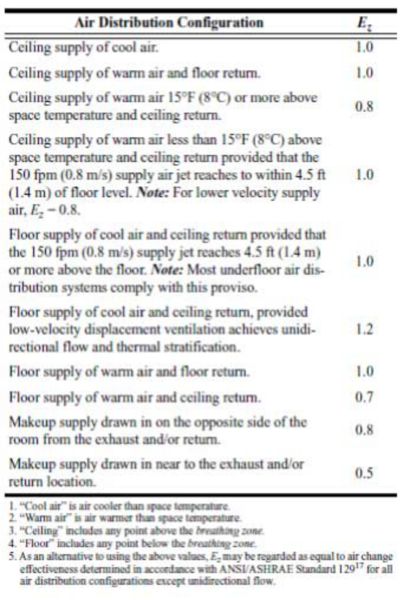
\includegraphics[width=0.9\textwidth, height=0.9\textheight, keepaspectratio=true]{media/image133.png}
\caption{Zone Air Distribution Effectiveness (Source: ASHRAE Standard 62.1-2010) \protect \label{fig:zone-air-distribution-effectiveness-source}}
\end{figure}

\paragraph{Field: Zone Air Distribution Effectiveness Schedule Name}\label{field-zone-air-distribution-effectiveness-schedule-name}

This optional field input points to a schedule with values of zone air distribution effectiveness. It provides a more flexible way of specifying zone air distribution effectiveness if it changes with time and/or system operating status and controls. If the schedule is specified, the zone air distribution effectiveness in cooling mode and heating mode will be ignored.

\paragraph{Field: Zone Secondary Recirculation Fraction}\label{field-zone-secondary-recirculation-fraction}

The non-negative numeric input for this field is the fraction of a zone's recirculation air that does not directly mix with the outdoor air. The zone secondary recirculation fraction Er is determined by the designer based on system configuration. For plenum return systems with secondary recirculation (e.g., fan-powered VAV with plenum return) Er is usually less than 1.0, although values may range from 0.1 to 1.2 depending upon the location of the ventilation zone relative to other zones and the air handler. For ducted return systems with secondary recirculation (e.g., fan-powered VAV with ducted return), Er is typically 0.0, while for those with system-level recirculation (e.g, dual-fan dual-duct systems with ducted return) Er is typically 1.0. For other system types, Er is typically 0.75. Minimum is 0.0, and default is 0.0 for single-path systems (also to maintain backward compatibility). For parallel fan-powered VAV systems, the secondary ventilation path only functions (Er \textgreater{} 0.0) when the fans in the VAV boxes operate, which is during heating. The local ventilation path and the benefits of secondary recirculation disappear during cooling, when the local parallel fans are off (Er = 0.0).

\paragraph{Field: Minimum Zone Ventilation
Efficiency}\label{field-minimum-zone-ventilation-efficiency}

This optional input sets a minimum on the ventilation efficiency for the zone. It is only used with the Ventilation Rate Procedure (VRP), single-path method. VRP should be chosen in Sizing System, System Outdoor Air Method = Standard62.1VentilationRateProcedure. Single-path method is indicated by leaving the previous input (Zone Secondary Recirculation Fraction) blank or setting it to 0.0. If the calculated value of ventilation efficiency for a zone is less than this value, it is raised to this minimum by raising the zone minimum air flow rate. This new value for zone minimum air flow rate then overrides other defaults and inputs in \hyperref[sizingzone]{Sizing:Zone}.

An example of this in an IDF context is shown:

\begin{lstlisting}

DesignSpecification:ZoneAirDistribution,
      CM DSZAD ZN_1_FLR_1_SEC_1,  !- Name
      1,                       !- Zone Air Distribution Effectiveness in Cooling Mode {dimensionless}
      1,                       !- Zone Air Distribution Effectiveness in Heating Mode {dimensionless}
      ;                        !- Zone Air Distribution Effectiveness Schedule Name
\end{lstlisting}

\subsection{Sizing:Parameters}\label{sizingparameters}

This object allows the user to specify global heating and cooling sizing ratios. These ratios will be applied at the zone level to all of the zone heating and cooling loads and air flow rates. These new loads and air flow rates are then used to calculate the system level flow rates and capacities and are used in all component sizing calculations.

The user can also specify the width (in load timesteps) of a moving average window which can be used to smooth the calculated zone design flow sequences. The use of this parameter is described below.

\subsubsection{Inputs}\label{inputs-2-010}

\paragraph{Field: Heating Sizing Factor}\label{field-heating-sizing-factor}

The global heating sizing ratio applied to all of the zone design heating loads and air flow rates.

\paragraph{Field: Cooling Sizing Factor}\label{field-cooling-sizing-factor}

The global cooling sizing ratio applied to all of the zone design cooling loads and air flow rates

\paragraph{Field: Timesteps in Averaging Window}\label{field-timesteps-in-averaging-window}

The number of load timesteps in the zone design flow sequence averaging window. The default is 1, in which case the calculated zone design flow rates are averaged over the load timestep.

The zone design air flow rate calculation is performed assuming a potentially infinite supply of heating or cooling air at a fixed temperature. Thus the calculated design air flow rate will always be able to meet any load or change in load no matter how large or abrupt. In reality air flow rates are limited by duct sizes and fan capacities. The idealized zone design flow calculation may result in unrealistically large flow rates, especially if the user is performing the sizing calculations using thermostat schedules with night setup or setback. The calculated zone design flow rates are always averaged over the load timestep. The user may want to perform a broader average to mitigate the effect of thermostat setup and setback and prevent the warm up or cool down flow rates from dominating the design flow rate calculation. Specifying the width of the averaging window allows the user to do this.

For example, if the load calculation timestep is 15 minutes and the user specifies the \emph{Timesteps in Averaging Window} to be 4, the zone design air flows will be averaged over a time period of 1 hour. Specifying 8 would result in averaging over a 2 hour period.

\subsubsection{Outputs}\label{outputs-009}

The sizing factors and the averaging window size are reported out on the \emph{eplusout.eio} file. An example is:

\begin{lstlisting}
! <Load Timesteps in Zone Design Calculation Averaging Window>, Value
 Timesteps in Averaging Window,    1
! <Heating Sizing Factor Information>, Sizing Factor ID, Value
 Heating Sizing Factor, Global,   1.3000
 Heating Sizing Factor, Zone SPACE1-1,   1.3000
 Heating Sizing Factor, Zone SPACE2-1,   1.3000
 Heating Sizing Factor, Zone SPACE3-1,   1.3000
 Heating Sizing Factor, Zone SPACE4-1,   1.3000
 Heating Sizing Factor, Zone SPACE5-1,   1.3000
! <Cooling Sizing Factor Information>, Sizing Factor ID, Value
 Cooling Sizing Factor, Global,   1.3000
 Cooling Sizing Factor, Zone SPACE1-1,   1.3000
 Cooling Sizing Factor, Zone SPACE2-1,   1.3000
 Cooling Sizing Factor, Zone SPACE3-1,   1.3000
 Cooling Sizing Factor, Zone SPACE4-1,   1.3000
 Cooling Sizing Factor, Zone SPACE5-1,   1.3000
\end{lstlisting}

\subsection{OutputControl:Sizing:Style}\label{outputcontrolsizingstyle}

As described early in the document (see: EnergyPlus Output Processing), the user may select the ``style'' for the sizing result files (epluszsz.\textless{}ext\textgreater{}, eplusssz.\textless{}ext\textgreater{}). This object applies to all sizing output files.

\begin{lstlisting}
OutputControl:Sizing:Style,
       \memo default style for the Sizing output files is comma -- this works well for
       \memo importing into spreadsheet programs such as Excel(tm) but not so well for word
       \memo processing progams -- there tab may be a better choice.  fixed puts spaces between
       \memo the "columns"
       \unique-object
   A1; \field Column Separator
       \required-field
       \type choice
       \key Comma
       \key Tab
       \key Fixed
\end{lstlisting}

\subsubsection{Inputs}\label{inputs-3-009}

\paragraph{Field: Column Separator}\label{field-column-separator-000}

For this field, the desired separator for columns is entered. ``Comma'' creates comma separated fields/columns in the outputs (eplus\textless{}sizing type\textgreater{}.csv files are created). ``Tab'' creates tab separated fields/columns in the outputs (eplus\textless{}sizing type\textgreater{}.tab files are created). ``Fixed'' creates space separated fields/columns in the outputs (eplus\textless{}sizing type\textgreater{}.txt files are created) but these are not necessarily lined up for easy printing.

Note that both tab and comma separated files easily import into Excel\textsuperscript{TM} or other spreadsheet programs. The tab delimited files can also be viewed by text editors, word processing programs and easily converted to ``tables'' within those programs.

\subsection{Sizing:Zone}\label{sizingzone}

The Sizing:Zone object provides the data needed to perform a zone design air flow calculation for a single zone. This calculation assumes a variable amount of supply air at a fixed temperature and humidity. The information needed consists of the zone inlet supply air conditions: temperature and humidity ratio for heating and cooling. The calculation is done for every design day included in the input. The maximum cooling load and air flow and the maximum heating load and air flow are then saved for the system level design calculations and for the component automatic sizing calculations.

The Sizing:Zone object is also the place where the user can specify the design outdoor air flow rate by referencing the name of a design specification outdoor air object. This can be specified in a number of ways (ref. \hyperref[designspecificationoutdoorair]{DesignSpecification:OutdoorAir}).This data is saved for use in the system sizing calculation or for sizing zone components that use outdoor air.

The user can also place limits on the heating and design cooling air flow rates. See \emph{~Heating Design Air Flow Method} and \emph{Cooling Design Air Flow Method} below and the explanations of the various heating and cooling flow input fields.

The user can ask the zone design calculation to take into account the effect of a Dedicated Outdoor Air System on the zone design loads and airflow rates. The design calculation will calculate the heat addition rate to the zone of an idealized SOA system and add or subtract the result from the total zone loads and flow rates.

Latent zone loads can also be calulated when specifying a \hyperref[field-zone-load-sizing-method]{Zone Load Sizing Method} other than Sensible Load Only No Latent Load. The design latent cooling and heating air flow will be calculated using the specified supply air humidity ratio and saved for further processing. Depending on the user choice for \emph{Zone Load Sizing Method},  the sensible, latent or largest load will determine the air flow rate used for the simulation. Care should be used to select appropriate values for \emph{Zone Cooling Design Supply Air Temperature}, \emph{Zone Heating Design Supply Air Temperature}, \emph{Zone Dehumidification Design Supply Air Humidity Ratio} and \emph{Zone Humidification Design Supply Air Humidity Ratio} as these values determine the zone sensible and latent mass flow rates. The larger the temperature difference, the smaller the air flow. Similarly, the larger the humidity ratio difference, the smaller the air flow. Coordinating these inputs will provide accurate results for air mass flow rate and which loads (i.e., sensible or latent) are largest.

\subsubsection{Inputs}\label{inputs-4-008}

\paragraph{Field: Zone Name}\label{field-zone-name-004}

The name of the Zone corresponding to this Sizing:Zone object. This is the zone for which the design air flow calculation will be made using the input data of this Sizing:Zone Object.

\paragraph{Field: Zone Cooling Design Supply Air Temperature Input Method}\label{field-zone-cooling-design-supply-air-temperature-input-method}

The input must be either \emph{SupplyAirTemperature} or \emph{TemperatureDifference}. \emph{SupplyAirTemperature} means that the user inputs from the fields of Zone Cooling Design Supply Air Temperature will be used to determine the zone cooling design air flow rates. \emph{TemperatureDifference} means that the user inputs from the fields of Zone Cooling Design Supply Air Temperature Difference will be used to determine the zone cooling design air flow rates.

\paragraph{Field: Zone Cooling Design Supply Air Temperature}\label{field-zone-cooling-design-supply-air-temperature}

The supply air temperature in degrees Celsius for the zone cooling design air flow rate calculation. Air is supplied to the zone at this temperature during the cooling design day simulation. The zone load is met by varying the zone air flow rate. The maximum zone flow rate is saved as the~ zone cooling design air flow rate. This field is only used when Zone Cooling Design Supply Air Temperature Input Method = \textbf{SupplyAirTemperature}. If the value entered for this parameter is less than zero, a warning message is produced so that the user will double check the input to make sure it is correct.

\paragraph{Field: Zone Cooling Design Supply Air Temperature Difference}\label{field-zone-cooling-design-supply-air-temperature-difference}

The temperature difference between cooling design supply air temperature and room air temperature in degrees Celsius for the zone cooling design air flow rate calculation. Air is supplied to the zone at this temperature during the cooling design day simulation. The zone load is met by varying the zone air flow rate. The maximum zone flow rate is saved as the zone cooling design air flow rate. This field is only used when Zone Cooling Design Supply Air Temperature Input Method = \textbf{TemperatureDifference}.

\paragraph{Field: Zone Heating Design Supply Air Temperature Input Method}\label{field-zone-heating-design-supply-air-temperature-input-method}

The input must be either \emph{SupplyAirTemperature} or \emph{TemperatureDifference}. \emph{SupplyAirTemperature} means that the user inputs from the fields of Zone Heating Design Supply Air Temperature will be used to determine the zone heating design air flow rates. \emph{TemperatureDifference} means that the user inputs from the fields of Zone Heating Design Supply Air Temperature Difference will be used to determine the zone heating design air flow rates.

\paragraph{Field: Zone Heating Design Supply Air Temperature}\label{field-zone-heating-design-supply-air-temperature}

The supply air temperature in degrees Celsius for the zone heating design air flow rate calculation. Air is supplied to the zone at this temperature during the heating design day simulation. The zone load is met by varying the zone air flow rate. The maximum zone flow rate is saved as the zone heating design air flow rate. This field is only used when Zone Heating Design Supply Air Temperature Input Method = \textbf{SupplyAirTemperature}. If the value entered for this parameter is less than zero, a warning message is produced so that the user will double check the input to make sure it is correct though other severe errors may happen before this happens.  In addition, this parameter must be greater than the Zone Cooling Design Supply Air Temperature field shown above.


\paragraph{Field: Zone Heating Design Supply Air Temperature Difference}\label{field-zone-heating-design-supply-air-temperature-difference}

The temperature difference between heating design supply air temperature and room air temperature in degrees Celsius for the zone heating design air flow rate calculation. Air is supplied to the zone at this temperature during the heating design day simulation. The zone load is met by varying the zone air flow rate. The maximum zone flow rate is saved as the zone heating design air flow rate. This field is only used when Zone Heating Design Supply Air Temperature Input Method = \textbf{TemperatureDifference}.

\paragraph{Field: Zone Cooling Design Supply Air Humidity Ratio}\label{field-zone-cooling-design-supply-air-humidity-ratio}

The humidity ratio in kilograms of water per kilogram of dry air of the supply air in the zone cooling design air flow rate calculation.

\paragraph{Field: Zone Heating Design Supply Air Humidity Ratio}\label{field-zone-heating-design-supply-air-humidity-ratio}

The humidity ratio in kilograms of water per kilogram of dry air of the supply air in the zone heating design air flow rate calculation.

\paragraph{Field: Design Specification Outdoor Air Object Name}\label{field-design-specification-outdoor-air-object-name-000}

This alpha field specifies the name of a \hyperref[designspecificationoutdoorair]{DesignSpecification:OutdoorAir} object which specifies the design outdoor air flow rate for the zone.

When a choice of IndoorAirQualityProcedure is entered in the Outdoor Air Method field of the \hyperref[designspecificationoutdoorair]{DesignSpecification:OutdoorAir} object, the design outdoor airflow rate is calculated based on the choice of Sum in the same field.

When a choice of ProportionalControlBasedOnDesignOccupancy or ProportionalControlBasedOnOccupancySchedule is entered, the design outdoor airflow rate is calculated based on equations specified in the "Proportional Control" section in the Engineering Reference.

\paragraph{Field: Zone Heating Sizing Factor}\label{field-zone-heating-sizing-factor}

This input is a zone level heating sizing ratio. The zone design heating air flow rates and loads will be multiplied by the number input in this field. This input overrides the building level sizing factor input in the \hyperref[sizingparameters]{Sizing:Parameters} object. And, of course, if this field is blank or zero, the global heating sizing factor from the \hyperref[sizingparameters]{Sizing:Parameters} object is used.

\paragraph{Field: Zone Cooling Sizing Factor}\label{field-zone-cooling-sizing-factor}

This input is a zone level cooling sizing ratio. The zone design cooling air flow rates and loads will be multiplied by the number input in this field. This input overrides the building level sizing factor input in the \hyperref[sizingparameters]{Sizing:Parameters} object. And, of course, if this field is blank or zero, the global cooling sizing factor from the \hyperref[sizingparameters]{Sizing:Parameters} object is used.

\paragraph{Field: Cooling Design Air Flow Method}\label{field-cooling-design-air-flow-method}

The input must be either \emph{Flow/Zone, DesignDay, or DesignDayWithLimit}. \emph{Flow/Zone} means that the program will use the input of the field \emph{Cooling Design Air Flow Rate} as the zone design cooling air flow rate. \emph{DesignDay} means the program will calculate the zone design cooling air flow rate using the Sizing:Zone input data and a design day simulation without imposing any limits other than those set by the minimum outside air requirements. \emph{DesignDayWithLimit} means that the maximum from \emph{Cooling Minimum Air Flow per Zone Floor Area} and \emph{Cooling Minimum Air Flow} will set a lower limit on the design maximum cooling air flow rate. The default method is \emph{DesignDay}: i.e., the program uses the calculated design values subject to ventilation requirements.

\paragraph{Field: Cooling Design Air Flow Rate}\label{field-cooling-design-air-flow-rate}

The design zone cooling air flow rate in cubic meters per second. This input is used if \emph{Cooling Design Air Flow Method} is specified as \emph{Flow/Zone}. This value will be multiplied by the global or zone sizing factor and by zone multipliers.

\paragraph{Field: Cooling Minimum Air Flow per Zone Floor Area}\label{field-cooling-minimum-air-flow-per-zone-floor-area}

The minimum zone cooling volumetric flow rate per square meter (units are m\(^{3}\)/s-m\(^{2}\)). This field is used when \emph{Cooling Design Air Flow Method} is specified as \emph{DesignDayWithLimit}. In this case it sets a lower bound on the zone design cooling air flow rate. In all cases the maximum flow derived from \emph{Cooling Minimum Air Flow per Zone Floor Area}, \emph{Cooling Minimum Air Flow}, \emph{Cooling Minimum Air Flow Fraction} and the design outdoor air flow rate (including VRP adjustments) is used to set a minimum supply air flow rate for the zone for VAV systems. The default is 0.000762, corresponding to 0.15 cfm/ft\(^{2}\). The applicable sizing factor is not applied to this value.

\paragraph{Field: Cooling Minimum Air Flow}\label{field-cooling-minimum-air-flow}

The minimum zone cooling volumetric flow rate in m\(^{3}\)/s. This field is used when \emph{Cooling Design Air Flow Method} is specified as \emph{DesignDayWithLimit}. In this case it sets a lower bound on the zone design cooling air flow rate.  In all cases the maximum flow derived from \emph{Cooling Minimum Air Flow per Zone Floor Area}, \emph{Cooling Minimum Air Flow}, \emph{Cooling Minimum Air Flow Fraction} and the design outdoor air flow rate (including VRP adjustments) is used to set a minimum supply air flow rate for the zone for VAV systems. The default is zero. The applicable sizing factor is not applied to this value.

\paragraph{Field: Cooling Minimum Air Flow Fraction}\label{field-cooling-minimum-air-flow-fraction}

The minimum zone design cooling volumetric flow rate expressed as a fraction of the zone design cooling volumetric flow rate.  In all cases the maximum flow derived from \emph{Cooling Minimum Air Flow per Zone Floor Area}, \emph{Cooling Minimum Air Flow}, \emph{Cooling Minimum Air Flow Fraction} and the design outdoor air flow rate (including VRP adjustments) is used to set a minimum supply air flow rate for the zone for VAV systems. The default is 0.2. This input is currently used in sizing the VAV air terminal unit and fan minimum flow rate. It does not currently affect other component autosizing.

\paragraph{Field: Heating Design Air Flow Method}\label{field-heating-design-air-flow-method}

The input must be either \emph{Flow/Zone, DesignDay, or DesignDayWithLimit}. \emph{Flow/Zone} means that the program will use the input of the field \emph{Heating Design Air Flow Rate} as the zone design heating air flow rate. \emph{DesignDay} means the program will calculate the zone design heating air flow rate using the Sizing:Zone input data and a design day simulation without imposing any limits other than those set by the minimum outside air requirements. \emph{DesignDayWithLimit} means that the maximum from \emph{Heating Maximum Air Flow per Zone Floor Area} and \emph{Heating Maximum Air Flow} will set a lower limit on the design maximum heating air flow rate. The default method is \emph{DesignDay}: i.e., the program uses the calculated design values subject to ventilation requirements.

\paragraph{Field: Heating Design Air Flow Rate}\label{field-heating-design-air-flow-rate}

The design zone heating air flow rate in cubic meters per second. This input is used if \emph{Heating Design Air Flow Method} is specified as \emph{Flow/Zone}. This value will be multiplied by the global or zone sizing factor and by zone multipliers.

\paragraph{Field: Heating Maximum Air Flow per Zone Floor Area}\label{field-heating-maximum-air-flow-per-zone-floor-area}

The maximum zone heating volumetric flow rate per square meter (units are m\(^{3}\)/s-m\(^{2}\)). This field is used when \emph{Heating Design Air Flow Method} is specified as \emph{DesignDayWithLimit}. In this case it sets an upper bound on the zone design heating air flow rate. For this and the next two input fields, the maximum flow derived from \emph{Heating Maximum Air Flow per Zone Floor Area}, \emph{Heating Maximum Air Flow}, and \emph{Heating Maximum Air Flow Fraction}~ is used to set a maximum heating supply air flow rate for the zone for VAV systems. The default is 0.002032, corresponding to 0.40 cfm/ft\(^{2}\). If the maximum heating design flow rate calculated using these input fields is greater than the design heating flow rate calculated during sizing, these input fields have no impact on sizing. It may be more appropriate to select only one of these three fields to calculate the maximum heating design flow rate (i.e., if one or more of these three fields is 0, it will not be used in calculating the maximum heating design flow rate).

\paragraph{Field: Heating Maximum Air Flow}\label{field-heating-maximum-air-flow}

The maximum zone heating volumetric flow rate in m\(^{3}\)/s. This field is used when \emph{Heating Design Air Flow Method} is specified as \emph{DesignDayWithLimit}. In this case it sets an upper bound on the zone design heating air flow rate. For this field and the two input fields just prior to and after this field,,the maximum flow derived from \emph{Heating Maximum Air Flow per Zone Floor Area}, \emph{Heating Maximum Air Flow}, and \emph{Heating Maximum Air Flow Fraction} is used to set a maximum heating supply air flow rate for the zone for VAV systems. The default is 0.1415762, corresponding to 300 cfm. If the maximum heating design flow rate calculated using these input fields is greater than the design heating flow rate calculated during sizing, these input fields have no impact on sizing. It may be more appropriate to select only one of these three fields to calculate the maximum heating design flow rate (i.e., if one or more of these three fields is 0, it will not be used in calculating the maximum heating design flow rate).

\paragraph{Field: Heating Maximum Air Flow Fraction}\label{field-heating-maximum-air-flow-fraction}

The maximum zone design heating volumetric flow rate expressed as a fraction of the zone design cooling volumetric flow rate. For this and the previous two input fields, the maximum flow derived from \emph{Heating Maximum Air Flow per Zone Floor Area}, \emph{Heating Maximum Air Flow}, and \emph{Heating Maximum Air Flow Fraction}~ is used to set a maximum heating supply air flow rate for the zone for VAV systems. The default is 0.3. If the maximum heating design flow rate calculated using these input fields is greater than the design heating flow rate calculated during sizing, these input fields have no impact on sizing. It may be more appropriate to select only one of these three fields to calculate the maximum heating design flow rate (i.e., if one or more of these three fields is 0, it will not be used in calculating the maximum heating design flow rate).

\paragraph{Field: Design Specification Zone Air Distribution Object Name}\label{field-design-specification-zone-air-distribution-object-name}

The name of the \hyperref[designspecificationzoneairdistribution]{DesignSpecification:ZoneAirDistribution} object, defining the air distribution effectiveness and secondary recirculation air fraction, that applies to the zone or zone list. This object may be used for the same zone in the \hyperref[controllermechanicalventilation]{Controller:MechanicalVentilation} object if no such \hyperref[designspecificationzoneairdistribution]{DesignSpecification:ZoneAirDistribution} object is specified.

\paragraph{Field: Account for Dedicated Outdoor Air System}\label{field-account-for-dedicated-outdoor-air-system}

This is a choice field with choices \emph{Yes} or \emph{No}. The default is \emph{No}. Choosing \emph{Yes} means that the zone sizing calculation will use the subsequent inputs to calculate the heat gain or loss (heat gains are positive, heat loss is negative) imposed on the zone by a Dedicated Outdoor Air System (DOAS). This heat gain is then added to the zone design heat gain for the zone and the zone design air flow rate is adjusted to meet the DOAS heat gain plus the zone design heat gain.

\paragraph{Field: Dedicated Outdoor Air System Control Strategy}\label{field-dedicated-outdoor-air-system-control-strategy}

This is a choice field with a choice of three ideal control strategies for the DOA system. The choices are \emph{NeutralSupplyAir}, \emph{NeutralDehumidifiedSupplyAir}, or \emph{ColdSupplyAir}. The default is \emph{NeutralSupplyAir}.

\emph{NeutralSupplyAir} implies that the ventilation air supplied to the zone will cause little heating or cooling. The air will be heated or cooled to keep it between the low and high temperature setpoints specified in the subsequent two fields. A good choice for these fields might be 21.1 and 23.9 degrees C.

\emph{NeutralDehumidifiedSupplyAir} means that the ventilation air will be cooled and dehumidified and then reheated to a neutral temperature. The ventilation air is cooled to the lower setpoint temperature (if necessary) and reheated to the upper setpoint temperature. A good choice for the setpoints would be 14.4 and 22.2 degrees C.

\emph{ColdSupplyAir} means that the ventilation air will be used to supply cooling to the zone. Cold outside air is heated to the upper setpoint; warm outside air is cooled to the lower setpoint. A good choice for the setpoints would be 12.2 and 14.4 degrees C.

\paragraph{Field: Dedicated Outdoor Air Low Temperature Setpoint for Design}\label{field-dedicated-outdoor-air-low-temperatue-setpoint-for-design}

The lower setpoint temperature to be used with the DOAS design control strategy. The units are degrees C. The default is autosized to the values given above for the three design control strategies.

\paragraph{Field: Dedicated Outdoor Air High Temperature Setpoint for Design}\label{field-dedicated-outdoor-air-high-temperature-setpoint-for-design}

The higher setpoint temperature to be used with the DOAS design control strategy. The units are degrees C. The default is autosized to the values given above for the three design control strategies.

\paragraph{Field: Zone Load Sizing Method}\label{field-zone-load-sizing-method}

Specifies the basis for sizing the zone supply air flow rate. Valid choices are Sensible Load, Latent Load, Sensible And Latent Load and Sensible Load Only No Latent Load. 
Zone latent loads will not be used during sizing only when Zone Load Sizing Method = Sensible Load Only No Latent Load (default). For this case the zone humidity level 
will float according to the fields Cooling and Heating Design Supply Air Humidity Ratio. For all other choices the zone humidity level will be controlled. Sensible Load will 
use zone sensible air flow rate for zone component sizing. Latent loads will also be reported during sizing. Latent Load will use zone latent air flow rate for zone component 
sizing. Sensible loads will also be reported during sizing. Sensible and Latent Load will use the larger of sensible and latent air flow rate for zone component sizing. Sensible 
Load Only No Latent Load or leaving this field blank will disable zone latent sizing and reporting. Latent loads will not be reported during sizing (reported as 0's).

\paragraph{Field: Zone Latent Cooling Design Supply Air Humidity Ratio Input Method}\label{field-zone-latent-cooling-design-supply-air-humidity-ratio-input-method}

Specifies the method for supply air humidity ratio used for latent sizing. Valid choices are SupplyAirHumidityRatio and HumidityRatioDifference (default). Use 
SupplyAirHumidityRatio to enter the humidity ratio when zone dehumidification is required. The supply air humidity ratio should be less than the zone humidity 
ratio at the zone thermostat and humidistat set point condition. Use HumidityRatioDifference to enter the difference in humidity ratio from the zone thermostat and 
humidistat set point condition.

\paragraph{Field: Zone Dehumidification Design Supply Air Humidity Ratio}\label{field-zone-dehumidification-design-supply-air-humidity-ratio}

Zone Dehumidification Design Supply Air Humidity Ratio (kgWater/kgDryAir) is only used when Zone Latent Cooling Design Supply Air Humidity Ratio Input Method = 
SupplyAirHumidityRatio. This input must be less than the zone humidity ratio at the humidistat set point so that dehumidification can occur.

\paragraph{Field: Zone Cooling Design Supply Air Humidity Ratio Difference}\label{field-zone-cooling-design-supply-air-humidity-ratio-difference}

Zone Dehumidification Design Supply Air Humidity Ratio Difference (kgWater/kgDryAir) is only used when Zone Latent Cooling Design Supply Air Humidity Ratio Input 
Method = HumidityRatioDifference. This input is a positive value and defines the difference between the zone humidity ratio at the thermostat and humidistat set point 
condition and the supply air humidity ratio entering the zone. 

\paragraph{Field: Zone Latent Heating Design Supply Air Humidity Ratio Input Method}\label{field-zone-latent-heating-design-supply-air-humidity-ratio-input-method}

Specifies the method for supply air humidity ratio used for latent sizing. Valid choices are SupplyAirHumidityRatio and HumidityRatioDifference (default). Use 
SupplyAirHumidityRatio to enter the humidity ratio when zone humidification is required. The supply air humidity ratio should be greater than the zone humidity 
ratio at the zone thermostat and humidistat set point condition. Use HumidityRatioDifference to enter the difference in humidity ratio from the zone thermostat and 
humidistat set point condition.

\paragraph{Field: Zone Humidification Design Supply Air Humidity Ratio}\label{field-zone-humidification-design-supply-air-humidity-ratio}

Zone Humidification Design Supply Air Humidity Ratio (kgWater/kgDryAir) is only used when Zone Latent Heating Design Supply Air Humidity Ratio Input Method = 
SupplyAirHumidityRatio. This input must be greater than the zone humidity ratio at the humidistat set point so that humidification can occur.

\paragraph{Field: Zone Heating Design Supply Air Humidity Ratio Difference}\label{field-zone-heating-design-supply-air-humidity-ratio-difference}

Zone Humidification Design Supply Air Humidity Ratio Difference (kgWater/kgDryAir) is only used when Zone Latent Heating Design Supply Air Humidity Ratio Input 
Method = HumidityRatioDifference. This input is a positive value and defines the difference between the zone humidity ratio at the thermostat and humidistat set point 
condition and the supply air humidity ratio entering the zone. 

\paragraph{Field: Zone Humidistat Dehumidification Set Point Schedule Name}\label{field-zone-humidistat-dehumidification-set-point-schedule-name}

Enter the zone relative humidity schedule used for zone latent cooling calculations. A zone humidistat will take priority over this input. This field is not used if Zone Load 
Sizing Method = Sensible Load Only No Latent Load or a zone humidistat is present. A default of 50.0 will be used if no schedule is provided and no humidistat is 
associated with this zone.

\paragraph{Field: Zone Humidistat Humidification Set Point Schedule Name}\label{field-zone-humidistat-humidification-set-point-schedule-name}

Enter the zone relative humidity schedule used for zone latent heating calculations. A zone humidistat will take priority over this input. This field is not used if Zone Load 
Sizing Method = Sensible Load Only No Latent Load or a zone humidistat is present. A default of 50.0 will be used if no schedule is provided and no humidistat is 
associated with this zone.

An IDF example:

\begin{lstlisting}

Sizing:Zone,
      SPACE5-1,                !- Name of a zone
      14.,                     !- Zone cooling design supply air temperature {C}
      50.,                     !- Zone heating design supply air temperature {C}
      0.009,                   !- Zone cooling design supply air humidity ratio {kg-H2O/kg-air}
      0.004,                   !- Zone heating design supply air humidity ratio {kg-H2O/kg-air}
      DSOA1,                   !- Design Specification Outdoor Air Object Name
      0.0,                     !- zone heating sizing factor
      0.0,                     !- zone cooling sizing factor
      designdaywithlimit,      !- Cooling Design Air Flow Method
      ,                        !- cooling design air flow rate {m3/s}
      ,                        !- Cooling Minimum Air Flow per zone area {m3/s-m2}
      ,                        !- Cooling Minimum Air Flow {m3/s}
      ,                        !- fraction of the cooling design air flow rate
      designday,               !- Heating Design Air Flow Method
      ,                        !- heating design air flow rate {m3/s}
      ,                        !- heating max air flow per zone area {m3/s-m2}
      ,                        !- heating max air flow {m3/s}
      ,                        !- fraction of the cooling design air flow rate
      DSZADO1,                 !- Design Specification Zone Air Distribution Object Name
      Yes,                     !- Account for Dedicated Outside Air System
      ColdSupplyAir,           !- Dedicated Outside Air System Control Strategy
      12.2,                    !- Dedicated Outside Air Low Setpoint for Design
      14.4,                    !- Dedicated Outside Air High Setpoint for Design
      Sensible And Latent Load, !- Zone Load Sizing Method
      HumidityRatioDifference, !- Zone Latent Cooling Design Supply Air Humidity Ratio Input Method
      ,                        !- Zone Dehumidification Design Supply Air Humidity Ratio
      0.005,                   !- Zone Cooling Design Supply Air Humidity Ratio Difference
      HumidityRatioDifference, !- Zone Latent Heating Design Supply Air Humidity Ratio Input Method
      ,                        !- Zone Humidification Design Supply Air Humidity Ratio
      0.005,                   !- Zone Heating Design Supply Air Humidity Ratio Difference
      ,                        !- Zone Humidistat Dehumidification Set Point Schedule Name
      ;                        !- Zone Humidistat Humidification Set Point Schedule Name

  DesignSpecification:OutdoorAir,
  DSOA1,                   !- Name
  SUM,                     !- Outdoor Air Method
  0.00236,                 !- Outdoor Air Flow per Person
  0.000305,                !- Outdoor Air Flow per Zone Floor Area
  0.0,                     !- Outdoor Air Flow per Zone
  0.0,                     !- Outdoor Air Flow Air Changes per Hour
  ;                        !- Outdoor Air Flow Rate Fraction Schedule Name

  DesignSpecification:ZoneAirDistribution,
      DSZADO1,                 !- Name
      1.0,                     !- Zone Air Distribution Effectiveness in Cooling Mode
      1.0,                     !- Zone Air Distribution Effectiveness in Heating Mode
      ,                        !- Zone Air Distribution Effectiveness Schedule Name
      0.3;                     !- Zone Secondary Recirculation Fraction
\end{lstlisting}

\subsubsection{Outputs}\label{outputs-1-007}

The zone design air flow rates and loads are output onto the local file ``epluszsz.\textless{}ext\textgreater{}'' where \textless{}ext\textgreater{} is the extension from the sizing style object (default is csv -- a comma separated file \emph{epluszsz.csv)}. The columns are clearly labeled. It will easily import into Excel or other spreadsheet program that accepts delimited files. All of these values are design air flow rates and loads \emph{calculated by the program}. No sizing factors have been applied.

The calculated zone design air flow rates and the user input or altered zone design air flow rates are also reported on the \emph{eplusout.eio} file. The values are printed out for each zone as comma separated records beginning with \emph{Zone Sizing}. Items output on the \emph{eio} file are: zone name, load type (heating or cooling), design load, calculated design air flow rate, user design air flow rate, design day name, time of peak, outside temperature at peak, outside humidity ratio at peak.

\subsection{DesignSpecification:ZoneHVAC:Sizing}\label{designspecificationzonehvacsizing}

This object is used to describe general sizing and scalable sizing methods which are referenced by zone HVAC equipment objects. It is optional input field in zone HVAC objects. If a name of this optional input is not specified or is blank then the sizing method or input specified in the parent object is used.~ If the name of this object is entered, then the values or method specified overrides the sizing method in the parent zone HVAC objects. This object is meant to provide scalable sizing method to users. The name of this object is an optional input field in the zoneHVAC objects. When this name in not specified in the zone HVAC object the sizing method or the value specified in the zone HVAC object will be used.

List of zoneHVAC objects than can reference this object include:

\begin{itemize}
\item
  \hyperref[zonehvacterminalunitvariablerefrigerantflow]{ZoneHVAC:TerminalUnit:VariableRefrigerantFlow}
\item
  \hyperref[zonehvacpackagedterminalairconditioner]{ZoneHVAC:PackagedTerminalAirConditioner}
\item
  \hyperref[zonehvacpackagedterminalheatpump]{ZoneHVAC:PackagedTerminalHeatPump}
\item
  \hyperref[zonehvacwatertoairheatpump]{ZoneHVAC:WaterToAirHeatPump}
\item
  \hyperref[zonehvacwindowairconditioner]{ZoneHVAC:WindowAirConditioner}
\item
  \hyperref[zonehvacunitheater]{ZoneHVAC:UnitHeater}
\item
  \hyperref[zonehvacunitventilator]{ZoneHVAC:UnitVentilator}
\item
  \hyperref[zonehvacfourpipefancoil]{ZoneHVAC:FourPipeFanCoil}
\item
  \hyperref[zonehvacventilatedslab]{ZoneHVAC:VentilatedSlab}
\item
  \hyperref[zonehvacevaporativecoolerunit]{ZoneHVAC:EvaporativeCoolerUnit}
\item
  \hyperref[zonehvacidealloadsairsystem]{ZoneHVAC:IdealLoadsAirSystem}
\end{itemize}

The sizing methods input fields available in this objects are for supply air flow and capacity for heating and cooling operating modes. Some zone HVAC equipment has single supply air flow rate input field that serves both cooling and heating operating modes.~ So entering either of the cooling or heating scalable sizing input field is sufficient.~ When there are separate input fields for cooling, heating, no-cooling, and no-heating operating modes, the corresponding input fields are specified.~ The child components supply air flow rate are also sized using scalable sizing methods specified in the parent objects. The methods allow users to enter a fixed or hard sized values, autosizable, or scalable sizing methods.~ Methods allowed for sizing supply air flow rates include: \emph{SupplyAirFlowRate}, \emph{FractionOfAutosizedCoolingAirflow}, \emph{FractionOfAutosizedHeatingAirflow}, \emph{FlowPerFloorArea, FlowPerCoolingCapacity}, and \emph{FlowPerHeatingCapacity}.~ The different sizing options are defined as follows:

\begin{itemize}
\item
  \textbf{SupplyAirFlowRate}: entered when it is intended that the user specified either hard value or the simulation engine autosize the supply air flow rates for cooling, heating, and no-cooling or no-heating operating modes.
\item
  \textbf{FlowPerFloorArea}: entered when it is intended that the simulation engine determine the supply air flow rates from the user specified \emph{supply air flow rates per unit floor area} and the zone floor area of the zone served by the zone HVAC equipment.
\item
  \textbf{FractionOfAutosizedCoolingAirflow}: entered when it is intended that the simulation engine determines the supply air flow rates from the user specified \emph{flow fraction} and \emph{autosized cooling design supply air flow rate}.
\item
  \textbf{FractionOfAutosizedHeatingAirflow}: entered when it is intended that the simulation engine determines the supply air flow rates from the user specified \emph{flow fraction} and \emph{autosized heating design supply air flow rate}.
\item
  \textbf{FlowPerCoolingCapacity}: entered when it is intended t that he simulation engine determines the supply air flow rates from the user specified \emph{supply air flow per cooling capacity value} and \emph{autosized cooling design capacity}.
\item
  \textbf{FlowPerHeatingCapacity}: entered when it is intended that the simulation engine determines the supply air flow rates from the user specified \emph{supply air flow per heating capacity value} and \emph{autosized heating design capacity}.
\end{itemize}

The~ Design Specification ZoneHVAC Sizing object also has input fields for sizing or scalable sizing of cooling and heating capacity. However, most of the parent zone HVAC objects do not have input fields for sizing capacities. So, the capacity scalable sizing fields in the parent objects are used for sizing child components capacity sizings.~ The scalable capacity sizing may be indirectly impacted by the scalable supply air flow rates sizing values. Moreover, the autosized cold water, hot water and steam flow rates in the parent zone HVAC objects (e.g. FanCoils, UnitHeaters, UnitVentilators, and VentilatedSlabs) and capacity in child components are determined using the scalable sizing methods. Sizing methods allowed for cooling and heating capacity include: \emph{CoolingDesignCapacity, HeatingDesignCapacity}, \emph{CapacityPerFloorArea, FractionOfAutosizedCoolingCapacity}, \emph{FractionOfAutosizedHeatingCapacity}.

\begin{itemize}
\item
  \textbf{CoolingDesignCapacity}: entered when it is intended that user specifies either a hard sized cooling capacity value or the simulation engine autosizes cooling capacity value for the cooling design capacity.
\item
  \textbf{HeatingDesignCapacity}: entered when it is intended that user specifies either a hard sized heating capacity value or the simulation engine autosized heating capacity value for the heating design capacity.
\item
  \textbf{CapacityPerFloorArea}: is entered when it is intended that the simulation engine determines the cooling or heating capacity from user specified capacity per floor area value and the floor area of the zone served by the zone HVAC equipment.
\item
  \textbf{FractionOfAutosizedCoolingCapacity}: entered when it is intended that the simulation engine sizes the cooling capacity from the user specified \emph{capacity fraction} and \emph{autosized cooling design capacity} value.
\item
  \textbf{FractionOfAutosizedHeatingCapacity}: entered when it is intended that the simulation engine sizes the heating capacity from the user specified \emph{capacity fraction} and \emph{autosized heating design capacity} value.
\end{itemize}

Description of the input fields of the design specification zone HVAC sizing object ``DesignSpecification:ZoneHVAC:Sizing'':

\subsubsection{Inputs}\label{inputs-5-007}

\paragraph{Field: Name}\label{designspecificationzonehvacsizing-field-name}

Unique identifier name of the DesignSpecification:ZoneHVAC:Sizing object. This sizing specification object referenced by a zone HVAC equipment whose design calculation will be made using the input data of this object.

\paragraph{Field: Cooling Design Air Flow Method}\label{field-cooling-design-air-flow-method-1}

The input of this field must be the method used to determine the cooling supply air volume flow rate. Input allowed is either \emph{None}, \emph{SupplyAirFlowRate}, \emph{FlowPerFloorArea}, \emph{FractionOfAutosizedCoolingAirflow}, or \emph{FlowPerCoolingCapacity}.~ None means cooling coil is not included in the zone HVAC equipment or this field may be left blank. \emph{SupplyAirFlowRate} means the user specifies the magnitude of supply air flow rate or the program calculates the design cooling supply air volume flow rate if autosize is specified. \emph{FlowPerFloorArea} means the program calculates the cooling supply air volume flow rate from zone floor area served by the zone HVAC unit and user specified \emph{Flow Per Floor Area} value. \emph{FractionOfAutosizedCoolingAirflow} means the program calculates the cooling supply air volume flow rate from user specified fraction and the autosized design cooling supply air volume flow rate value determined by the simulation. FlowPerCoolingCapacity means the supply air volume is calculated from user specified flow per cooling capacity and design cooling capacity determined by the simulation. The default method is \emph{SupplyAirFlowRate}.

\paragraph{Field: Cooling Design Supply Air Flow Rate \{m3/s\}}\label{field-cooling-design-supply-air-flow-rate-m3s}

Enter the magnitude of the cooling supply air volume flow rate in m3/s. This input is an alternative to using the program auto-calculated value. This input is a required field when the Cooling Design air Flow Method is \emph{SupplyAirFlowRate}. This field may be left blank if a cooling coil is not included in the zone HVAC equipment. This input field is also autosizable.

\paragraph{Field: Cooling Design Supply Air Flow Rate Per Floor Area \{m3/s-m2\}}\label{field-cooling-design-supply-air-flow-rate-per-floor-area-m3s-m2}

Enter the cooling supply air volume flow rate per zone conditioned floor area in m3/s-m2. This field is required field when the Cooling Design air Flow Method is \emph{FlowPerFloorArea}. This field may be left blank if a cooling coil is not included in the zone HVAC equipment or the Cooling Design Air Flow Method is not \emph{FlowPerFloorArea}. The program calculates the cooling supply air volume flow rate from the zone conditioned floor area served by the zone HVAC equipment and the flow per unit area value specified by the user. Zone sizing object (\hyperref[sizingzone]{Sizing:Zone}) is not required.

\paragraph{Field: Fraction of Autosized Cooling Design Supply Air Flow Rate}\label{field-fraction-of-autosized-cooling-design-supply-air-flow-rate}

Enter the cooling supply air volume flow rate as a fraction of the autosized cooling supply air flow rate. This input field is required when the Cooling Design air Flow Method is \emph{FractionOfAutosizedCoolingAirflow}. This input field may be left blank if a cooling coil is not included in the zone HVAC equipment or the Cooling Design air Flow Method is not \emph{FractionOfAutosizedCoolingAirflow}. The program calculates the cooling supply air volume flow rate from the design autosized cooling supply air flow rate and user specified fraction. Zone sizing object (\hyperref[sizingzone]{Sizing:Zone}) is required.

\paragraph{Field: Cooling Design Supply Air Flow Rate Per Unit Cooling Capacity \{m3/s-W\}}\label{field-cooling-design-supply-air-flow-rate-per-unit-cooling-capacity-m3s-w}

Enter the cooling supply air volume flow rate per unit cooling capacity in m3/s-W. This input field is required when the Cooling Design air Flow Method is \emph{FlowPerCoolingCapacity}. This field may be left blank if a cooling coil is not included in the zone HVAC equipment or the Cooling Design air Flow Method is not \emph{FlowPerCoolingCapacity}. The program calculates the cooling supply air volume flow rate from the design autosized cooling capacity and user specified flow per cooling capacity value. Zone sizing object (\hyperref[sizingzone]{Sizing:Zone}) is required.

\paragraph{Field: Supply Air Flow Rate Method When No Cooling or Heating is Required}\label{field-supply-air-flow-rate-method-when-no-cooling-or-heating-is-required}

Enter the method used to determine the supply air volume flow rate when No Cooling or Heating is required. Inputs allowed are \emph{None}, \emph{SupplyAirFlowRate}, \emph{FlowPerFloorArea}, \emph{FractionOfAutosizedCoolingAirflow}, and \emph{FractionOfAutosizedHeatingAirflow.} \emph{None} is used when a cooling or heating coil is not included in the zone HVAC equipment or this field may be left blank. \emph{SupplyAirFlowRate} means user specifies the magnitude of supply air flow rate or the program calculates the design supply air volume flow rate if autosize is specified. \emph{FlowPerFloorArea} means the program calculates the supply air volume flow rate from the zone floor area served by the zone HVAC unit and Flow Per Floor Area value specified by user. \emph{FractionOfAutosizedCoolingAirflow} means the program calculates the supply air volume flow rate from user specified fraction and autosized design cooling supply air volume flow rate value determined by the program. FractionOfAutosizedHeatingAirflow means the program calculates the supply air volume flow rate from user specified fraction and autosized heating supply air flow rate value determined by the program. The default method is \emph{SupplyAirFlowRate}.

\paragraph{Field: Supply Air Flow Rate When No Cooling or Heating is Required \{m3/s\}}\label{field-supply-air-flow-rate-when-no-cooling-or-heating-is-required-m3s}

Enter the magnitude of the supply air volume flow rate when no cooling or heating is required in m3/s. This input is an alternative to using the program auto-calculated value. This input is a required field when the Supply Air Flow Rate Method When No Cooling or Heating is Required is \emph{SupplyAirFlowRate}. This field may be left blank if a cooling coil is not included in the zone HVAC equipment. This input field is also autosizable.

\paragraph{Field: Supply Air Flow Rate Per Floor Area When No Clg or Htg is Required~ \{m3/s-m2\}}\label{field-supply-air-flow-rate-per-floor-area-when-no-clg-or-htg-is-required-m3s-m2}

Enter the magnitude of supply air volume flow rate per zone floor area in m3/s-m2. This input is a required field when Supply Air ~Flow Rate Method When No Cooling or Heating is Required is \emph{FlowPerFloorArea}. The program calculates the supply air flow rate when no cooling or heating is required from user specified flow per floor area and the zone area served by current zoneHVAC equipment.

\paragraph{~Field: Fraction of Design Cooling Supply Air Flow Rate When No Clg or Htg Required}\label{field-fraction-of-design-cooling-supply-air-flow-rate-when-no-clg-or-htg-required}

Enter the fraction of supply air volume flow rate as a fraction of the autosized cooling supply air flow rate. This input field is required field when Supply Air Flow Rate Method When No Cooling or Heating is Required is \emph{FractionOfAutosizedCoolingAirflow}.~ The program calculates the supply air flow rate when no cooling or heating is required from user specified fraction and the design cooling autosized supply air flow rate.

\paragraph{Field: Fraction of Design Heating Supply Air Flow Rate When No Clg or Htg Required}\label{field-fraction-of-design-heating-supply-air-flow-rate-when-no-clg-or-htg-required}

Enter the fraction of supply air volume flow rate as a fraction of the autosized cooling supply air flow rate. This input field is required field when Supply Air Flow Rate Method When No Cooling or Heating is Required is \emph{FractionOfAutosizedHeatingAirflow}.~ The program calculates the supply air flow rate when no cooling or heating is required from user specified fraction and the design heating autosized supply air flow rate.

\paragraph{Field: Heating Design Air Flow Method}\label{field-heating-design-air-flow-method-1}

The input of this field must be the method used to determine the heating supply air volume flow rate. Input allowed is either \emph{None}, \emph{SupplyAirFlowRate}, \emph{FlowPerFloorArea}, \emph{FractionOfAutosizedCoolingAirflow}, or \emph{FlowPerCoolingCapacity}.~ \emph{None} means heating coil is not included in the zone HVAC equipment or this field may be left blank. \emph{SupplyAirFlowRate} means the user specifies the magnitude of supply air flow rate or the program calculates the design heating supply air volume flow rate if autosize is specified. \emph{FlowPerFloorArea} means the program calculates the heating supply air volume flow rate from zone floor area served by the zone HVAC unit and user specified \emph{Flow Per Floor Area} value. \emph{FractionOfAutosizedHeatingAirflow} means the program calculates the heating supply air volume flow rate from user specified fraction and the autosized design heating supply air volume flow rate value determined by the simulation. \emph{FlowPerHeatingCapacity} means the supply air volume is calculated from user specified flow per heating capacity and design heating capacity determined by the simulation. The default method is \emph{SupplyAirFlowRate}.

\paragraph{Field: Heating Design Supply Air Flow Rate \{m3/s\}}\label{field-heating-design-supply-air-flow-rate-m3s}

Enter the magnitude of the heating supply air volume flow rate in m3/s. This input is an alternative to using the program auto-calculated value. This input is a required field when the Heating Design air Flow Method is \emph{SupplyAirFlowRate}. This field may be left blank if a heating coil is not included in the zone HVAC equipment. This input field is also autosizable.

\paragraph{Field: Heating Design Supply Air Flow Rate Per Floor Area \{m3/s-m2\}}\label{field-heating-design-supply-air-flow-rate-per-floor-area-m3s-m2}

Enter the heating supply air volume flow rate per zone conditioned floor area in m3/s-m2. This field is required field when the Heating Design air Flow Method is \emph{FlowPerFloorArea}. This field may be left blank if a heating coil is not included in the zone HVAC equipment or the Heating Design Air Flow Method is not \emph{FlowPerFloorArea}. The program calculates the heating supply air volume flow rate from the zone conditioned floor area served by the zone HVAC equipment and the flow per unit area value specified by the user.

\paragraph{Field: Fraction of Autosized Heating Design Supply Air Flow Rate}\label{field-fraction-of-autosized-heating-design-supply-air-flow-rate}

Enter the heating supply air volume flow rate as a fraction of the autosized heating supply air flow rate. This input field is required when the Heating Design air Flow Method is \emph{FractionOfAutosizedHeatingAirflow}. This input field may be left blank if a heating coil is not included in the zone HVAC equipment or the Heating Design air Flow Method is not \emph{FractionOfAutosizedHeatingAirflow}. The program calculates the heating supply air volume flow rate from the design autosized heating supply air flow rate and user specified fraction.

\paragraph{Field: Heating Design Supply Air Flow Rate Per Unit Heating Capacity \{m3/s-W\}}\label{field-heating-design-supply-air-flow-rate-per-unit-heating-capacity-m3s-w}

Enter the heating supply air volume flow rate per unit heating capacity in m3/s-W. This input field is required when the Heating Design air Flow Method is \emph{FlowPerHeatingCapacity}. This field may be left blank if a cooling coil is not included in the zone HVAC equipment or the Heating Design air Flow Method is not \emph{FlowPerHeatingCapacity}. The program calculates the heating supply air volume flow rate from the design autosized heating capacity and user specified flow per unit heating capacity value.

\paragraph{Field Cooling Design Capacity Method}\label{field-cooling-design-capacity-method}

Enter the method used to determine the cooling design capacity for scalable sizing. Input allowed is either \emph{None}, \emph{CoolingDesignCapacity}, \emph{CapacityPerFloorArea}, and \emph{FractionOfAutosizedCoolingCapacity}. None is used when a cooling coil is not included in the Zone HVAC equipment or this field may be left blank. If this input field is left blank, then the design cooling capacity is set to zero. \emph{CoolingDesignCapacity} means user specifies the magnitude of cooling capacity or the program calculates the design cooling capacity if autosize is specified. \emph{CapacityPerFloorArea} means the program calculates the design cooling capacity from user specified cooling capacity per floor area and floor area of the zone served by the HVAC unit. \emph{FractionOfAutosizedCoolingCapacity} means the program calculates the design cooling capacity from user specified fraction and the auto-sized design cooling capacity. The default method is \emph{CoolingDesignCapacity}.

\paragraph{Field: Cooling Design Capacity \{W\}}\label{field-cooling-design-capacity-w}

Enter the magnitude of the cooling capacity in Watts. This input is an alternative to using the program auto-calculated cooling capacity value. This input is a required field when the Cooling Design Capacity Method is \emph{CoolingDesignCapacity}. This field may be left blank if a cooling coil is not included in the zone HVAC equipment or alternative method is specified. This input field is autosizable. Design day sizing run must be specified.

\paragraph{Field: Cooling Design Capacity Per Floor Area \{W/m2\}}\label{field-cooling-design-capacity-per-floor-area-wm2}

Enter the cooling capacity per unit floor area in m3/s-m2. This field is required field when the Cooling Design Capacity Method is \emph{CapacityPerFloorArea}. This field may be left blank if a cooling coil is not included in the zone HVAC equipment or the Cooling Design Capacity Method is not \emph{CapacityPerFloorArea}. The program calculates the cooling capacity from floor area of the zone served by the zone HVAC equipment and the cooling capacity per unit floor area value specified by the user.

\paragraph{Field: Fraction of Autosized Cooling Design Capacity}\label{field-fraction-of-autosized-cooling-design-capacity}

Enter the cooling capacity as a fraction of the autosized cooling capacity. This input field is required when the Cooling Design Capacity Method is \emph{FractionOfAutosizedCoolingCapacity}. This input field may be left blank if a cooling coil is not included in the zone HVAC equipment or the Cooling Design Capacity Method is not \emph{FractionOfAutosizedCoolingCapacity}. The program calculates the cooling capacity from the design autosized cooling capacity and user specified fraction. Design day sizing run must be specified.

\paragraph{Field: Heating Design Capacity Method}\label{field-heating-design-capacity-method}

Enter the method used to determine the heating design capacity for scalable sizing. Input allowed is either \emph{None}, \emph{HeatingDesignCapacity}, \emph{CapacityPerFloorArea}, and \emph{FractionOfAutosizedHeatingCapacity}. None is used when a heating coil is not included in the Zone HVAC equipment or this field may be left blank. If this input field is left blank, then the design heating capacity is set to zero. \emph{HeatingDesignCapacity} means user specifies the magnitude of heating capacity or the program calculates the design heating capacity if autosize is specified. \emph{CapacityPerFloorArea} means the program calculates the design heating capacity from user specified heating capacity per floor area and floor area of the zone served by the HVAC unit. \emph{FractionOfAutosizedHeatingCapacity} means the program calculates the design heating capacity from user specified fraction and the auto-sized design heating capacity. The default method is \emph{HeatingDesignCapacity}.

\paragraph{Field: Heating Design Capacity \{W\}}\label{field-heating-design-capacity-w}

Enter the magnitude of the heating capacity in Watts. This input is an alternative to using the program auto-calculated heating capacity value. This input is a required field when the Heating Design Capacity Method is \emph{HeatingDesignCapacity}. This field may be left blank if a heating coil is not included in the zone HVAC equipment or alternative method is specified. This input field is autosizable. Design day sizing run must be specified.

\paragraph{Field: Heating Design Capacity Per Floor Area \{W/m2\}}\label{field-heating-design-capacity-per-floor-area-wm2}

Enter the heating capacity per unit floor area in m3/s-m2. This field is required field when the Heating Design Capacity Method is \emph{CapacityPerFloorArea}. This field may be left blank if a heating coil is not included in the zone HVAC equipment or the Heating Design Capacity Method is not \emph{CapacityPerFloorArea}. The program calculates the heating capacity from floor area of the zone served by the zone HVAC equipment and the heating capacity per unit floor area value specified by the user.

\paragraph{Field: Fraction of Autosized Heating Design Capacity}\label{field-fraction-of-autosized-heating-design-capacity}

Enter the heating capacity as a fraction of the autosized heating capacity. This input field is required when the Heating Design Capacity Method is \emph{FractionOfAutosizedHeatingCapacity}. This input field may be left blank if a heating coil is not included in the zone HVAC equipment or the Heating Design Capacity Method is not \emph{FractionOfAutosizedHeatingCapacity}. The program calculates the heating capacity from the design autosized cooling capacity and user specified fraction. Design day sizing run must be specified.

\begin{lstlisting}

  DesignSpecification:ZoneHVAC:Sizing,
      VRFDesignSpec1,          !- Name
      SupplyAirFlowRate,       !- Cooling Design Air Flow Method
      autosize,                !- Cooling Design Supply Air Flow Rate
      ,                        !- Cooling Design Supply Air Flow Rate Per Floor Area
      ,                        !- Fraction of Autosized Cooling Design Supply Air Flow Rate
      ,                        !- Cooling Design Supply Air Flow Rate Per Unit of Capacity {m3/s-W}
      SupplyAirFlowRate,       !- Supply Air Flow Rate Method When No Cooling or Heating is Required
      autosize,                !- Supply Air Flow Rate When No Cooling or Heating is Required
      ,                        !- Supply Air Flow Rate Per Floor Area When No Clg or Htg is Required
      ,                     !- Fraction of Autosized Design Cooling Supply Air Flow Rate When No Clg or Htg
      ,                     !- Fraction of Autosized Design Heating Supply Air Flow Rate When No Clg or Htg
      SupplyAirFlowRate,       !- Heating Design Air Flow Method
      autosize,                !- Heating Design Supply Air Flow Rate
      ,                        !- Heating Design Supply Air Flow Rate Per Floor Area
      ,                        !- Fraction of Autosized Heating Design Supply Air Flow Rate
      ,                        !- Heating Design Supply Air Flow Rate Per Unit of Heating Capacity
      CoolingDesignCapacity,   !- Cooling Design Capacity Method
      autosize,                !- Cooling Design Capacity {W}
      ,                        !- Cooling Design Capacity Per Floor Area {W/m2}
      ,                        !- Fraction of Autosized Cooling Design Capacity {-}
      HeatingDesignCapacity,   !- Heating Design Capacity Method
      autosize,                !- Heating Design Capacity {W}
      ,                        !- Heating Design Capacity Per Floor Area {W/m2}
      ;                        !- Fraction of Autosized Cooling Design Capacity {-}

    DesignSpecification:ZoneHVAC:Sizing,
      VRFDesignSpec2,          !- Name
      FlowPerFloorArea,        !- Cooling Design Air Flow Method
      ,                        !- Cooling Design Supply Air Flow Rate
      3.6311418E-03,           !- Cooling Design Supply Air Flow Rate Per Floor Area
      ,                        !- Fraction of Autosized Cooling Design Supply Air Flow Rate
      ,                        !- Cooling Design Supply Air Flow Rate Per Unit of Capacity {m3/s-W}
      FlowPerFloorArea,        !- Supply Air Flow Rate Method When No Cooling or Heating is Required
      ,                        !- Supply Air Flow Rate When No Cooling or Heating is Required
      3.6311418E-03,           !- Supply Air Flow Rate Per Floor Area When No Clg or Htg is Required
      ,                     !- Fraction of Autosized Design Cooling Supply Air Flow Rate When No Clg or Htg
      ,                     !- Fraction of Autosized Design Heating Supply Air Flow Rate When No Clg or Htg
      FlowPerFloorArea,        !- Heating Design Air Flow Method
      ,                        !- Heating Design Supply Air Flow Rate
      3.6311418E-03,           !- Heating Design Supply Air Flow Rate Per Floor Area
      ,                        !- Fraction of Autosized Heating Design Supply Air Flow Rate
      ,                        !- Heating Design Supply Air Flow Rate Per Unit of Heating Capacity
      CoolingDesignCapacity,   !- Cooling Design Capacity Method
      autosize,                !- Cooling Design Capacity {W}
      ,                        !- Cooling Design Capacity Per Floor Area {W/m2}
      ,                        !- Fraction of Autosized Cooling Design Capacity {-}
      HeatingDesignCapacity,   !- Heating Design Capacity Method
      autosize,                !- Heating Design Capacity {W}
      ,                        !- Heating Design Capacity Per Floor Area {W/m2}
      ;                        !- Fraction of Autosized Cooling Design Capacity {-}

  DesignSpecification:ZoneHVAC:Sizing,
      VRFDesignSpec3,          !- Name
      FractionOfAutosizedCoolingAirflow,  !- Cooling Design Air Flow Method
      ,                        !- Cooling Design Supply Air Flow Rate
      ,                        !- Cooling Design Supply Air Flow Rate Per Floor Area
      0.5,                     !- Fraction of Autosized Cooling Design Supply Air Flow Rate
      ,                        !- Cooling Design Supply Air Flow Rate Per Unit of Capacity {m3/s-W}
    FractionOfAutosizedCoolingAirflow, !- Supply Air Flow Rate Method When No Cooling or Heating is Required
      ,                        !- Supply Air Flow Rate When No Cooling or Heating is Required
      ,                        !- Supply Air Flow Rate Per Floor Area When No Clg or Htg is Required
      0.5,                 !- Fraction of Autosized Design Cooling Supply Air Flow Rate When No Clg or Htg
      ,                    !- Fraction of Autosized Design Heating Supply Air Flow Rate When No Clg or Htg
      FractionOfAutosizedHeatingAirflow,  !- Heating Design Air Flow Method
      ,                        !- Heating Design Supply Air Flow Rate
      ,                        !- Heating Design Supply Air Flow Rate Per Floor Area
      0.5,                     !- Fraction of Autosized Heating Design Supply Air Flow Rate
      ,                        !- Heating Design Supply Air Flow Rate Per Unit of Heating Capacity
      CoolingDesignCapacity,   !- Cooling Design Capacity Method
      autosize,                !- Cooling Design Capacity {W}
      ,                        !- Cooling Design Capacity Per Floor Area {W/m2}
      ,                        !- Fraction of Autosized Cooling Design Capacity {-}
      HeatingDesignCapacity,   !- Heating Design Capacity Method
      autosize,                !- Heating Design Capacity {W}
      ,                        !- Heating Design Capacity Per Floor Area {W/m2}
      ;                        !- Fraction of Autosized Cooling Design Capacity {-}

  DesignSpecification:ZoneHVAC:Sizing,
      VRFDesignSpec4,          !- Name
      FlowPerCoolingCapacity,  !- Cooling Design Air Flow Method
      ,                        !- Cooling Design Supply Air Flow Rate
      ,                        !- Cooling Design Supply Air Flow Rate Per Floor Area
      ,                        !- Fraction of Autosized Cooling Design Supply Air Flow Rate
      2.9541628E-05,           !- Cooling Design Supply Air Flow Rate Per Unit of Capacity {m3/s-W}
    FractionOfAutosizedHeatingAirflow, !- Supply Air Flow Rate Method When No Cooling or Heating is Required
      ,                        !- Supply Air Flow Rate When No Cooling or Heating is Required
      ,                        !- Supply Air Flow Rate Per Floor Area When No Clg or Htg is Required
      ,                    !- Fraction of Autosized Design Cooling Supply Air Flow Rate When No Clg or Htg
      0.413231177,         !- Fraction of Autosized Design Heating Supply Air Flow Rate When No Clg or Htg
      FlowPerHeatingCapacity,  !- Heating Design Air Flow Method
      ,                        !- Heating Design Supply Air Flow Rate
      ,                        !- Heating Design Supply Air Flow Rate Per Floor Area
      ,                        !- Fraction of Autosized Heating Design Supply Air Flow Rate
      2.9541628E-05,           !- Heating Design Supply Air Flow Rate Per Unit of Heating Capacity
      CoolingDesignCapacity,   !- Cooling Design Capacity Method
      autosize,                !- Cooling Design Capacity {W}
      ,                        !- Cooling Design Capacity Per Floor Area {W/m2}
      ,                        !- Fraction of Autosized Cooling Design Capacity {-}
      HeatingDesignCapacity,   !- Heating Design Capacity Method
      autosize,                !- Heating Design Capacity {W}
      ,                        !- Heating Design Capacity Per Floor Area {W/m2}
      ;                        !- Fraction of Autosized Cooling Design Capacity {-}
\end{lstlisting}

\subsection{DesignSpecification:AirTerminal:Sizing}\label{designspecificationairterminalsizing}

This object modifies the sizing of an air loop terminal unit. It may be referenced by a \hyperref[zonehvacairdistributionunit]{ZoneHVAC:AirDistributionUnit} object. The values specified here are applied to the base sizing results from the corresponding \hyperref[sizingzone]{Sizing:Zone} inputs. Any given DesignSpecification:AirTerminal:Sizing object may be used by multiple terminal units with similar characteristics.

\subsubsection{Inputs}\label{inputs-52-007}

\paragraph{Field: Name}\label{designspecificationairterminalsizing-field-name}

Name of the design specification air terminal sizing object. This name may be referenced by a \hyperref[zonehvacairdistributionunit]{ZoneHVAC:AirDistributionUnit} object.

\paragraph{Field: Fraction of Design Sensible Cooling Load}\label{fraction-of-design-sensible-cooling-load}

The fraction of the design sensible cooling load to be met by this terminal unit. This fraction is applied after the Zone Cooling Sizing Factor (see \hyperref[sizingzone]{Sizing:Zone}).

\paragraph{Field: Cooling Design Supply Air Temperature Difference Ratio}\label{cooling-design-supply-air-temperature-difference-ratio}

This ratio adjusts the supply air temperature difference used to calculate the cooling design supply air flow rate for this terminal unit.

\paragraph{Field: Fraction of Design Sensible Heating Load}\label{fraction-of-design-sensible-heating-load}

The fraction of the design sensible heating load to be met by this terminal unit. This fraction is applied after the Zone Heating Sizing Factor (see \hyperref[sizingzone]{Sizing:Zone}).

\paragraph{Field: Heating Design Supply Air Temperature Difference Ratio}\label{heating-design-supply-air-temperature-difference-ratio}

This ratio adjusts the supply air temperature difference used to calculate the heating design supply air flow rate for this terminal unit.

\paragraph{Field: Fraction of Minimum Outdoor Air Flow}\label{fraction-of-minimum-outdoor-air-requirement}

The fraction of the zone minimum outdoor air requirement to be met by this terminal unit.

An IDF example:

\begin{lstlisting}

  DesignSpecification:AirTerminal:Sizing,
    Recirculation System A Terminal Sizing, !- Name
    0.6,                     !- Fraction of Design Cooling Load
    0.8,                     !- Cooling Design Supply Air Temperature Difference Ratio
    1.0,                     !- Fraction of Design Heating Load
    1.0,                     !- Heating Design Supply Air Temperature Difference Ratio
    0.0;                     !- Fraction of Minimum Outdoor Air Flow
\end{lstlisting}

\subsection{Sizing:System}\label{sizingsystem}

The Sizing:System object contains the input needed to perform a central forced air system design air flow, heating capacity, and cooling capacity calculation for a system serving one or more zones. The information needed consists of the outside environmental conditions and the design supply air temperatures, outdoor air flow rate, and minimum system air flow ratio.

The outside conditions come from the design days in the input. A system sizing calculation is performed for every design day in the input file and the resulting maximum heating and cooling air flow rates and capacities are saved for use in the component sizing calculations.

Supply air conditions are specified by inputting a supply air temperature for cooling, a supply air temperature for heating, and a preheat temperature.

The system sizing calculation sums the zone design air flow rates to obtain a system supply air flow rate. The design conditions and the outdoor air flow rate are used to calculate a design mixed air temperature. The temperature plus the design supply air temperatures allows the calculation of system design heating and cooling capacities.

\subsubsection{Inputs}\label{inputs-6-006}

\paragraph{Field: AirLoop Name}\label{field-airloop-name}

The name of the \hyperref[airloophvac]{AirLoopHVAC} corresponding to this Sizing:System object. This is the air system for which the design calculation will be made using the input data of this Sizing:System Object.

\paragraph{Field: Type of Load to Size On}\label{field-type-of-load-to-size-on}

The user specified type of load on which to size the central system. The choices are \emph{Sensible}, \emph{Latent}, \emph{Total} and \emph{VentilationRequirement}. \emph{Sensible}, \emph{Latent} and \emph{Total} mean that the central system supply air flow rate will be determined by combining the zone design air flow rates, which have been calculated to meet the zone sensible and latent loads from the design days. Latent sizing requires the the zones connected to this air system be sized for latent loads, otherwise sizing will use sensible loads. Additionally, if zone latent sizing is performed and zone latent loads do not exceed zone sensible loads, sizing will use sensible loads. If any zone latent load exceeds a zone's sensible load, latent sizing will be performed. \emph{VentilationRequirement} means that the central system supply air flow rate will be determined by the system ventilation requirement. In addition \emph{Sensible} tells the program to size the central cooling coil using entering air flow rate and air conditions at the sensible load peak; \emph{Total} indicates that the program should size the central cooling coil at the air flow rate and conditions at the total load peak. The central heating coil is always sized at the conditions at the peak sensible heating load.

\paragraph{Field: Design Outdoor Air Flow Rate}\label{field-design-outdoor-air-flow-rate}

The design outdoor air flow rate in cubic meters per second. Generally this should be the minimum outdoor air flow. It is used for both heating and cooling design calculations. The assumption for cooling is that any outdoor air economizer will be closed. If \emph{Autosize} is input the outdoor air flow rate will be taken from the sum of the zone outdoor air flow rates or calculated based on the System Outdoor Air Method selection (field below).

\paragraph{Field: Central Heating Maximum System Air Flow Ratio}\label{field-central-heating-maximum-system-air-flow-ratio}

The ratio of the maximum system air flow rate for heating to the maximum system air flow rate. The value must be between 0 and 1. For constant volume systems the ratio should be set to 1. This ratio should be set to reflect what the user expects the system flow rate to be when maximum heating demand occurs. This ratio is used in calculating the central system heating capacity. Thus if the system is VAV with the zone VAV dampers held at minimum flow when there is a zone heating demand, this ratio should be set to the minimum flow ratio. If the zone VAV dampers are reverse action and can open to full flow to meet heating demand, this ratio should be set to 1. The default is set to 0.5, reflecting the fact that VAV dampers are typically not allowed to fully open during heating.

This field can be set to \emph{AutoSize}.  When automatically calculated, the ratio is determined from the system heating design flow rate divided by the main (which is usually the max of heating and cooling design flow rates) design flow rate.  The design flow rates are also adjusted to be more accurate by examining each of the air terminals attached to the air system and summing the heating and maximum flow rates.

\paragraph{Field: Preheat Design Temperature}\label{field-preheat-design-temperature}

The design air temperature exiting the preheat coil (if any) in degrees Celsius.

\paragraph{Field: Preheat Design Humidity Ratio}\label{field-preheat-design-humidity-ratio}

The design humidity ratio exiting the preheat coil (if any) in kilograms of water per kilogram of dry air. (kgWater/kgDryAir)

\paragraph{Field: Precool Design Temperature}\label{field-precool-design-temperature}

The design air temperature exiting the precooling coil (if any) in degrees Celsius.

\paragraph{Field: Precool Design Humidity Ratio}\label{field-precool-design-humidity-ratio}

The design humidity ratio exiting the precooling coil (if any) in kilograms of water per kilogram of dry air. (kgWater/kgDryAir)

\paragraph{Field: Central Cooling Design Supply Air Temperature}\label{field-central-cooling-design-supply-air-temperature}

The design supply air temperature for cooling in degrees Celsius. This should be the temperature of the air exiting the central cooling coil.

\paragraph{Field: Central Heating Design Supply Air Temperature}\label{field-central-heating-design-supply-air-temperature}

The design supply air temperature for heating in degrees Celsius. This can be either the reset temperature for a single duct system or the actual hot duct supply air temperature for dual duct systems. It should be the temperature at the exit of the main heating coil. This value is also used for the sizing of zone equipment (e.g., reheat coil) for the system embedded with central heating coils, but it is not used if there is no central heating coil in the system.

\paragraph{Field: Type of Zone Sum to Use}\label{field-type-of-zone-sum-to-use}

If the input is \emph{coincident} the central system air flow rate will be sized on the sum of the coincident zone air flow rates. If the input is \emph{noncoincident} the central system air flow rate will be sized on the sum of the noncoincident zone air flow rates. The default is noncoincident.

\paragraph{Field: 100\% Outdoor Air in Cooling}\label{field-100-outdoor-air-in-cooling}

Entering \emph{Yes} means the system will be sized for cooling using 100\% outdoor air. Entering \emph{No} means the system will be sized for cooling using minimum outside air (the default).

\paragraph{Field: 100\% Outdoor Air in Heating}\label{field-100-outdoor-air-in-heating}

Entering \emph{Yes} means the system will be sized for heating using 100\% outdoor air. Entering \emph{No} means the system will be sized for heating using minimum outside air (the default).

\paragraph{Field: Central Cooling Design Supply Air Humidity Ratio}\label{field-central-cooling-design-supply-air-humidity-ratio}

The design humidity ratio in kilograms of water per kilogram of dry air at the exit of the central cooling coil. The default is 0.008 (kgWater/kgDryAir).

\paragraph{Field: Central Heating Design Supply Air Humidity Ratio}\label{field-central-heating-design-supply-air-humidity-ratio}

The design humidity ratio in kilograms of water per kilogram of dry air at the exit of the central heating coil. This value is also used for the sizing of zone equipment (e.g., reheat coil) for the system embedded with central heating coils, but it is not used if there is no central heating coil in the system. The default is 0.008 (kgWater/kgDryAir).

\paragraph{Field: Cooling Supply Air Flow Rate Method}\label{field-cooling-supply-air-flow-rate-method}

The input of this field must be the method used to determine the airloop cooling supply air volume flow rate. The input must be either, \emph{DesignDay}, \emph{Flow/System,} \emph{FlowPerFloorArea}, \emph{FractionOfAutosizedCoolingAirflow}, or \emph{FlowPerCoolingCapacity}. \emph{DesignDay} means the program will calculate the system design cooling supply air volume flow rate using the System Sizing input data and a design day simulation. \emph{Flow/System} means that the program will use the input of the field \emph{Cooling Design Air Flow Rate} as the system design cooling supply air volume flow rate. \emph{FlowPerFloorArea} means the program calculates the cooling supply air volume flow rate from zone floor area served by the airloop and user specified \emph{Flow Per Floor Area} value. \emph{FractionOfAutosizedCoolingAirflow} means the program calculates the cooling supply air volume flow rate from user specified fraction and the autosized design cooling supply air volume flow rate value determined by the simulation. \emph{FlowPerCoolingCapacity} means the supply air volume is calculated from user specified flow per cooling capacity and design cooling capacity determined by the simulation. The default method is \emph{DesignDay}: i.e., the program uses the calculated design values.

\paragraph{Field: Cooling Supply Air Flow Rate}\label{field-cooling-supply-air-flow-rate}

The design system cooling air flow rate in cubic meters per second. This input is an alternative to using the program autocalculated value. This input is used if Cooling Supply Air Flow Rate Method is Flow/System. This value will \emph{not} be multiplied by any sizing factor or by zone multipliers. If using zone multipliers, this value must be large enough to serve the multiplied zones.

\paragraph{Field: Cooling Supply Air Flow Rate Per Floor Area \{m3/s-m2\}}\label{field-cooling-supply-air-flow-rate-per-floor-area-m3s-m2}

Enter the cooling supply air volume flow rate per zone conditioned floor area in m3/s-m2. This field is required field when the Cooling Supply Air Flow Rate Method is \emph{FlowPerFloorArea}. This field may be left blank if a cooling coil is not included in the airloop or the Cooling Supply Air Flow Rate Method is not \emph{FlowPerFloorArea}. The program calculates the cooling supply air volume flow rate from the cooled floor area served by the air loop and the \emph{Flow Per Unit Area} value specified by the user.

\paragraph{Field: Cooling Fraction of Autosized Cooling Design Supply Air Flow Rate}\label{field-cooling-fraction-of-autosized-cooling-design-supply-air-flow-rate}

Enter the cooling supply air volume flow rate as a fraction of the airloop autosized cooling supply air flow rate. This input field is required when the Cooling Supply Air Flow Rate Method is \emph{FractionOfAutosizedCoolingAirflow}. This input field may be left blank if a cooling coil is not included in the airloop or the Cooling Supply Air Flow Rate Method is not \emph{FractionOfAutosizedCoolingAirflow}. The program calculates the cooling supply air volume flow rate from the design autosized cooling supply air flow rate and user specified fraction.

\paragraph{Field: Cooling Supply Air Flow Rate Per Unit Cooling Capacity \{m3/s-W\}}\label{field-cooling-supply-air-flow-rate-per-unit-cooling-capacity-m3s-w}

Enter the cooling supply air volume flow rate per unit cooling capacity in m3/s-W. This input field is required when the Cooling Supply Air Flow Rate Method is \emph{FlowPerCoolingCapacity}. This field may be left blank if a cooling coil is not included in the airloop or the Cooling Supply Air Flow Rate Method is not \emph{FlowPerCoolingCapacity}. The program calculates the airloop cooling supply air volume flow rate from the design autosized cooling capacity and user specified \emph{Flow Per Cooling Capacity} value.

\paragraph{Field: Heating Supply Air Flow Rate Method}\label{field-heating-supply-air-flow-rate-method}

The input of this field must be the method used to determine the airloop heating supply air volume flow rate. The input must be either, \emph{DesignDay}, \emph{Flow/System,} \emph{FlowPerFloorArea}, \emph{FractionOfAutosizedHeatingAirflow}, \emph{FractionOfAutosizedCoolingAirflow} or \emph{FlowPerHeatingCapacity}. \emph{DesignDay} means the program will calculate the system design heating supply air volume flow rate using the System Sizing input data and a design day simulation. \emph{Flow/System} means that the program will use the input of the field \emph{Heating Design Air Flow Rate} as the system design heating supply air volume flow rate. \emph{FlowPerFloorArea} means the program calculates the system heating supply air volume flow rate from zone floor area served by the airloop and user specified \emph{Flow Per Floor Area} value. \emph{FractionOfAutosizedHeatingAirflow} means the program calculates the system heating supply air volume flow rate from user specified fraction and the autosized system design heating supply air volume flow rate value determined by the simulation. \emph{FractionOfAutosizedCoolingAirflow} means the program calculates the system heating supply air volume flow rate from user specified fraction and the autosized system design cooling supply air volume flow rate value determined by the simulation. \emph{FlowPerHeatingCapacity} means the system heating supply air volume is calculated from user specified flow per heating capacity and design heating capacity determined by the simulation. The default method is \emph{DesignDay}: i.e., the program uses the calculated design values.

\paragraph{Field: Heating Supply Air Flow Rate}\label{field-heating-supply-air-flow-rate}

The design system heating air flow rate in cubic meters per second. This input is an alternative to using the program autocalculated value. This input is used if Heating Supply Air Flow Rate Method is Flow/System. This value will \emph{not} be multiplied by any sizing factor or by zone multipliers. If using zone multipliers, this value must be large enough to serve the multiplied zones.

\paragraph{Field: Heating Supply Air Flow Rate Per Floor Area \{m3/s-m2\}}\label{field-heating-supply-air-flow-rate-per-floor-area-m3s-m2}

Enter the heating supply air volume flow rate per zone conditioned floor area in m3/s-m2. This field is required field when the Heating Supply Air Flow Rate Method is \emph{FlowPerFloorArea}. This field may be left blank if a heating coil is not included in the airloop or the Heating Supply Air Flow Rate Method is not \emph{FlowPerFloorArea}. The program calculates the heating supply air volume flow rate from the heated or cooled floor area served by the air loop and the \emph{Flow Per Unit Area} value specified by the user.

\paragraph{Field: Heating Fraction of Autosized Heating Supply Air Flow Rate}\label{field-heating-fraction-of-autosized-heating-supply-air-flow-rate}

Enter the heating supply air volume flow rate as a fraction of the airloop autosized heating supply air flow rate. This input field is required when the Heating Supply Air Flow Rate Method is \emph{FractionOfAutosizedHeatingAirflow}. This input field may be left blank if heating coil is not included in the airloop or the Heating Supply Air Flow Rate Method is not \emph{FractionOfAutosizedHeatingAirflow}. The program calculates the heating supply air volume flow rate from the design autosized heating supply air flow rate and user specified fraction.

\paragraph{Field: Heating Fraction of Autosized Cooling Supply Air Flow Rate}\label{field-heating-fraction-of-autosized-cooling-supply-air-flow-rate}

Enter the heating supply air volume flow rate as a fraction of the airloop autosized cooling supply air flow rate. This input field is required when the Heating Supply Air Flow Rate Method is \emph{FractionOfAutosizedCoolingAirflow}. This input field may be left blank if heating coil is not included in the airloop or the Heating Supply Air Flow Rate Method is not \emph{FractionOfAutosizedCoolingAirflow}. The program calculates the heating supply air volume flow rate from the design autosized cooling supply air flow rate and user specified fraction.

\paragraph{Field: Heating Design Supply Air Flow Rate Per Unit Heating Capacity \{m3/s-W\}}\label{field-heating-design-supply-air-flow-rate-per-unit-heating-capacity-m3s-w-1}

Enter the heating supply air volume flow rate per unit heating capacity in m3/s-W. This input field is required when the Heating Design air Flow Method is \emph{FlowPerCoolingCapacity}. This field may be left blank if a heating coil is not included in the airloop or the Heating Design air Flow Method is not \emph{FlowPerHeatingCapacity}. The program calculates the airloop heating supply air volume flow rate from the design autosized heating capacity and user specified \emph{Flow Per Heating Capacity} value.

\paragraph{Field: System Outdoor Air Method}\label{field-system-outdoor-air-method-000}

The method used to calculate the system minimum outdoor air flow. The three choices are ZoneSum, Standard62.1VentilationRateProcedure (VRP), and Standard62.1SimplifiedProcedure (SP). ZoneSum sums the outdoor air flows across all zones served by the system. VRP uses the multi-zone equations defined in ASHRAE Standard 62.1 to calculate the system outdoor air flow. VRP considers zone air distribution effectiveness and zone diversification of outdoor air fractions. VRP may also adjust autosized air terminal maximum and minimum supply flow rates if needed to ensure adequate outdoor air flow rate to each zone. SP is similar to VRP and was introduced in ASHRAE Standard 62.1-2019. The main difference with VRP is that it uses a simplified approach to calculate a system's ventilation efficiency which is in turn used to calculate the system outdoor air flow. Additionally, when set to autosize, the minimum (primary) air flow (or air flow fraction) of these types of air terminals will be calculated following SP: \hyperref[airterminalsingleductvavnoreheat]{AirTerminal:SingleDuct:VAV:NoReheat} (\emph{Constant Minimum Air Flow Fraction} or \emph{Fixed Minimum Air Flow Fraction}), 
\hyperref[airterminalsingleductvavreheat]{AirTerminal:SingleDuct:VAV:Reheat} (\emph{Constant Minimum Air Flow Fraction} or \emph{Fixed Minimum Air Flow Fraction}), \hyperref[airterminalsingleductseriespiureheat]{AirTerminal:SingleDuct:SeriesPIU:Reheat} (\emph{Minimum Primary Air Flow Fraction}), 
 \hyperref[airterminalsingleductparallelpiureheat]{AirTerminal:SingleDuct:ParallelPIU:Reheat}(\emph{Minimum Primary Air Flow Fraction}).

\paragraph{Field: Zone Maximum Outdoor Air Fraction}\label{field-zone-maximum-outdoor-air-fraction-000}

This positive numeric input is the zone maximum outdoor air fraction. For an air loop, when a zone requires outdoor air higher than the user specified Zone Maximum Outdoor Air Fraction, the zone supply air flow will be increased to cap the outdoor air fraction at the maximum value. This allows the system level outdoor air flow to be reduced while the total supply air flow increases. Valid values are from 0 to 1.0. Default is 1.0 which indicates zones can have 100\% outdoor air maintaining backward compatibility. This input work for constant volume air systems, single and dual duct VAV systems.

\paragraph{Field Cooling Design Capacity Method}\label{field-cooling-design-capacity-method-1}

Enter the method used to determine the cooling design capacity for scalable sizing. Input allowed is either \emph{None}, \emph{CoolingDesignCapacity}, \emph{CapacityPerFloorArea}, and \emph{FractionOfAutosizedCoolingCapacity}. None is used when a cooling coil is not included in the airloop. If this input field is left blank, or None is specified, then the autosized design cooling capacity determined by the program is used. \emph{CoolingDesignCapacity} means user specifies the magnitude of cooling capacity or the program calculates the design cooling capacity if autosize is specified. \emph{CapacityPerFloorArea} means the program calculates the design cooling capacity from user specified cooling capacity per floor area and floor area of the zones served by the airloop. \emph{FractionOfAutosizedCoolingCapacity} means the program calculates the design cooling capacity from user specified fraction and the auto-sized design cooling capacity. If the value this input field is blank or specified as None, then the next three input fields are not required. The default method is \emph{CoolingDesignCapacity}.

\paragraph{Field: Cooling Design Capacity \{W\}}\label{field-cooling-design-capacity-w-1}

Enter the magnitude of the cooling capacity in Watts. This input is an alternative to using the program auto-calculated cooling capacity value. This input is a required field when the Cooling Design Capacity Method is \emph{CoolingDesignCapacity}. This field may be left blank if a cooling coil is not included in the air loop or alternative method is specified. This input field is autosizable.

\paragraph{Field: Cooling Design Capacity Per Floor Area \{W/m2\}}\label{field-cooling-design-capacity-per-floor-area-wm2-1}

Enter the cooling capacity per unit floor area in m3/s-m2. This field is required field when the Cooling Design Capacity Method is \emph{CapacityPerFloorArea}. This field may be left blank if a cooling coil is not included in the airloop or the Cooling Design Capacity Method is not \emph{CapacityPerFloorArea}. The program calculates the cooling capacity from floor area of the zones served by the airloop and the cooling capacity per unit floor area value specified by the user.

\paragraph{Field: Fraction of Autosized Cooling Design Capacity}\label{field-fraction-of-autosized-cooling-design-capacity-1}

Enter the cooling capacity as a fraction of the autosized cooling capacity. This input field is required when the Cooling Design Capacity Method is \emph{FractionOfAutosizedCoolingCapacity}. This input field may be left blank if a cooling coil is not included in the zone HVAC equipment or the Cooling Design Capacity Method is not \emph{FractionOfAutosizedCoolingCapacity}. The program calculates the cooling capacity from the design autosized cooling capacity and user specified fraction. Design day sizing run must be specified.

\paragraph{Field: Heating Design Capacity Method}\label{field-heating-design-capacity-method-1}

Enter the method used to determine the heating design capacity for scalable sizing. Input allowed is either \emph{None}, \emph{HeatingDesignCapacity}, \emph{CapacityPerFloorArea}, and \emph{FractionOfAutosizedHeatingCapacity}. \emph{None} is used when a heating coil is not included in the airloop. If this input field is left blank, then the autosized design heating capacity determined by the program is used. \emph{HeatingDesignCapacity} means user specifies the magnitude of heating capacity or the program calculates the design heating capacity if autosize is specified. \emph{CapacityPerFloorArea} means the program calculates the design heating capacity from user specified heating capacity per floor area and floor area of the zones served by the airllop. \emph{FractionOfAutosizedHeatingCapacity} means the program calculates the design heating capacity from user specified fraction and the auto-sized design heating capacity. If the value this input field is blank or specified as None, then the next three input fields are not required. The default method is \emph{HeatingDesignCapacity}.

\paragraph{Field: Heating Design Capacity \{W\}}\label{field-heating-design-capacity-w-1}

Enter the magnitude of the heating capacity in Watts. This input is an alternative to using the program auto-calculated heating capacity value. This input is a required field when the Heating Design Capacity Method is \emph{HeatingDesignCapacity}. This field may be left blank if a heating coil is not included in the airloop or alternative method is specified. This input field is autosizable.

\paragraph{Field: Heating Design Capacity Per Floor Area \{W/m2\}}\label{field-heating-design-capacity-per-floor-area-wm2-1}

Enter the heating capacity per unit floor area in m3/s-m2. This field is required field when the Heating Design Capacity Method is \emph{CapacityPerFloorArea}. This field may be left blank if a heating coil is not included in the airloop or the Heating Design Capacity Method is not \emph{CapacityPerFloorArea}. The program calculates the heating capacity from floor area of the zones served by the airloop and the heating capacity per unit floor area value specified by the user.

\paragraph{Field: Fraction of Autosized Heating Design Capacity}\label{field-fraction-of-autosized-heating-design-capacity-1}

Enter the heating capacity as a fraction of the autosized heating capacity. This input field is required when the Heating Design Capacity Method is FractionOfAutosizedHeatingCapacity. This input field may be left blank if heating coil is not included in the airloop or the Heating Design Capacity Method is not FractionOfAutosizedHeatingCapacity. The program calculates the heating capacity from the design autosized cooling capacity and user specified fraction.

\paragraph{Field: Central Cooling Capacity Control Method}\label{field-central-cooling-capacity-control-method}

Specifies how the central cooling coil will be controlled, which affects the coil sizing calculation. There are 4 choices: VAV, Bypass, VT, and OnOff. Choose VAV if the cooling output is controlled by varying the air flow. Bypass should be chosen if the capacity is controlled by bypassing a variable fraction of the mixed air around the coil face. VT indicates that cooling coil output is controlled by varying the coil exit temperature while the flow rate is constant. And OnOff means that the cooling output is controlled by cycling the air flow.

\paragraph{Field: Occupant Diversity}\label{occupant-diversity}

The Occupant Diversity (D) as defined in ASHRAE Standard 62.1. The Occupant Diversity is a ratio of the expected peak population to the design zone population for all zones attached to the air system. If left blank or set to autosize, EnergyPlus will calculate it by using the people schedules and design levels included in the model.

An IDF example:

\begin{lstlisting}

Sizing:System,
  VAV Sys 1,               !- AirLoop Name
  sensible,                !- Type of Load to Size On
  autosize,                !- Design Outdoor Air Flow Rate {m3/s}
  0.3,                     !- Minimum System Air Flow Ratio
  4.5,                     !- Preheat Design Temperature {C}
  .008,                    !- Preheat Design Humidity Ratio {kgWater/kgDryAir}
  11.0,                    !- Precool Design Temperature {C}
  .008,                    !- Precool Design Humidity Ratio {kgWater/kgDryAir}
  12.8,                    !- Central Cooling Design Supply Air Temperature {C}
  16.7,                    !- Central Heating Design Supply Air Temperature {C}
  noncoincident,           !- Sizing Option
  no,                      !- 100% Outdoor Air in Cooling
  no,                      !- 100% Outdoor Air in Heating
  0.008,                   !- Central Cooling Design Supply Air Humidity Ratio {kgWater/kgDryAir}
  0.008,                   !- Central Heating Design Supply Air Humidity Ratio {kgWater/kgDryAir}
  designday,               !- Cooling Supply Air Flow Rate Method
  0,                       !- Cooling Supply Air Flow Rate {m3/s}
  ,                        !- Cooling Supply Air Flow Rate Per Floor Area {m3/s-m2}
  ,                        !- Cooling Fraction of Autosized Cooling Supply Air Flow Rate {-}
  ,                        !- Cooling Supply Air Flow Rate Per Unit Cooling Capacity {m3/s-W}
  designday,               !- Heating Supply Air Flow Rate Method
  0,                       !- Heating Supply Air Flow Rate {m3/s}
  ,                        !- Heating Supply Air Flow Rate Per Floor Area {m3/s-m2}
  ,                        !- Heating Fraction of Autosized Heating Supply Air Flow Rate {-}
  ,                        !- Heating Fraction of Autosized Cooling Supply Air Flow Rate {-}
  ,                        !- Heating Supply Air Flow Rate Per Unit Heating Capacity {m3/s-W}
  ZoneSum,                 !- System Outdoor Air Method
  0.5,                     !- Zone Maximum Outdoor Air Fraction
  CoolingDesignCapacity,   !- Cooling Design Capacity Method
  autosize,                !- Cooling Design Capacity {W}
  ,                        !- Cooling Design Capacity Per Floor Area {W/m2}
  ,                        !- Fraction of Autosized Cooling Design Capacity {-}
  HeatingDesignCapacity,   !- Heating Design Capacity Method
  autosize,                !- Heating Design Capacity {W}
  ,                        !- Heating Design Capacity Per Floor Area {W/m2}
  ;                        !- Fraction of Autosized Cooling Design Capacity {-}
\end{lstlisting}

\subsubsection{Outputs}\label{outputs-2-006}

The system design air flow rates and heating and cooling capacities are output onto the local file ``eplusssz.\textless{}ext\textgreater{}'' where \textless{}ext\textgreater{} is the extension from the sizing style object (default is csv -- a comma separated file \emph{eplusssz.csv)}. The columns are clearly labeled. It will easily import into Excel or other spreadsheet program that accepts delimited files. The results are calculated values and do not include any user input system flow rates.

The calculated system design air flow rates and the user input system design air flow rates are also reported on the \emph{eplusout.eio} file. The values are printed out for each system as comma separated records beginning with \emph{System Sizing}. An example is:

\begin{lstlisting}
! <System Sizing Information>c++, System Name, Field Description, Value
 System Sizing, VAV SYS 1, Calculated Cooling Design Air Flow Rate [m3/s],   1.3194
 System Sizing, VAV SYS 1, User Cooling Design Air Flow Rate [m3/s],   1.5000
 System Sizing, VAV SYS 1, Calculated Heating Design Air Flow Rate [m3/s],  0.90363
 System Sizing, VAV SYS 1, User Heating Design Air Flow Rate [m3/s],   1.0000
\end{lstlisting}

\subsection{Sizing:Plant}\label{sizingplant}

The Sizing:Plant object contains the input needed for the program to calculate plant loop flow rates and equipment capacities when autosizing. This information is initially used by components that use water for heating or cooling such as hot or chilled water coils to calculate their maximum water flow rates. These flow rates are then summed for use in calculating the Plant Loop flow rates.

The program will size any number of chilled water, hot water, condenser water and other plant loops. There should be one Sizing:Plant object for each plant loop that is to be autosized.

\subsubsection{Inputs}\label{inputs-7-006}

\paragraph{Field: Plant or Condenser Loop Name}\label{field-plant-or-condenser-loop-name}

The name of a Plant Loop or Condenser Loop object corresponding to this Sizing:Plant object. This is the plant loop for which this data will be used for calculating the loop flow rate.

\paragraph{Field: Loop Type}\label{field-loop-type}

The possible inputs are \emph{Heating, Steam, Cooling,} or \emph{Condenser}.

\paragraph{Field: Design Loop Exit Temperature}\label{field-design-loop-exit-temperature}

The water temperature in degrees Celsius at the exit of the supply side of the plant loop, Thus this is the temperature of the water supplied to the inlet of chilled or hot water coils and other equipment that places loads on a plant loop.

\paragraph{Field: Loop Design Temperature Difference}\label{field-loop-design-temperature-difference}

The design temperature rise (for cooling or condenser loops) or fall (for heating loops) in degrees Celsius across the demand side of a plant loop.~ This temperature difference is used by component models to determine flow rates required to meet design capacities.~ Larger values lead to smaller design flow rates.

\paragraph{Field: Sizing Option}\label{field-sizing-option}

This field is optional. This field controls how concurrence issues impact the plant loop design flow rate. If it is not used then the program uses noncoincident method, which is the historical behavior prior to version 8.3. There are two choices, noncoincident and coincident. The use of Coincident sizing option requires that the \hyperref[simulationcontrol]{SimulationControl} object be set to YES for the input field called Do HVAC Sizing Simulation for Sizing Periods.

\paragraph{Field: Zone Timesteps in Averaging Window}\label{field-zone-timesteps-in-averaging-window}

This field is optional and is only used if the preceding field is set to Coincident. This is the number of zone timesteps used in a moving average to determine the design flow rate from HVAC Sizing Simulation approach. This allows using a broader average over time when using coincident plant sizing. This is similar in concept to the similar field in \hyperref[sizingparameters]{Sizing:Parameters} which specifies the averaging window for zone loads. The default is 1.

\paragraph{Field: Coincident Sizing Factor Mode}\label{field-coincident-sizing-factor-mode}

This field is only used if the sizing option is set to Coincident. This field controls the behavior of coincident sizing with respect to what, if any, sizing factor should be applied to further modify the flow rate measured while running HVAC Sizing Simulations. There are four options. Enter the keword None to use the raw value for flow rate without modification. Enter the keyword GlobalHeatingSizingFactor to modify the flow by the sizing factor entered in the object called \hyperref[sizingparameters]{Sizing:Parameters} for heating. Enter the keyword GlobalCoolingSizingFactor to modify the flow by the sizing factor entered in the object called \hyperref[sizingparameters]{Sizing:Parameters} for cooling. Enter the keyword LoopComponentSizingFactor to modify the flow by a sizing factor determined from the combination of component-level sizing factors in the associated plant loop.

An IDF example:

\begin{lstlisting}

Sizing:Plant,
     Chilled Water Loop, ! name of loop
     Cooling,            ! type of loop
     7.22,               ! chilled water supply temperature
     6.67,               ! chilled water delta T
  NonCoincident,      !- Sizing Option
  1,                  !- Zone Timesteps in Averaging Window
  GlobalCoolingSizingFactor; !- Coincident Sizing Factor Mode
\end{lstlisting}

\subsubsection{Outputs}\label{outputs-3-004}

The loop flow rates are reported on the \emph{eplusout.eio} file along with the component sizing results.

When coincident plant sizing method is used, the eio file contains special summary report with various details and interim values from the calculations, under the following record header: ! , Plant Loop Name, Sizing Pass \{\#\}, Measured Mass Flow\{kg/s\}, Measured Demand \{W\}, Demand Calculated Mass Flow\{kg/s\}, Sizes Changed \{Yes/No\}, Previous Volume Flow Rate \{m3/s\}, New Volume Flow Rate \{m3/s\}, Demand Check Applied \{Yes/No\}, Sizing Factor \{\}, Normalized Change \{\}, Specific Heat\{\}.
